\documentclass[11pt]{beamer}
\usetheme{Madrid}
\usepackage[utf8]{inputenc}
\usepackage{amsmath}
\usepackage{amsfonts}
\usepackage{amssymb}
\usepackage{multicol}

\usepackage[normalem]{ulem}

%\usepackage{caption}

%trim={<left> <lower> <right> <upper>}

\author{S-P. Hallsj{\"o}}
\date{}
\title{Baby MIND}
\subtitle{Plots for meeting}
%\setbeamercovered{transparent} 
%\setbeamertemplate{navigation symbols}{} 
%\logo{} 
\institute[U. of G.]{University of Glasgow} 
%\titlegraphic{\includegraphics[scale=0.5]{baseImages/ExperPartPhys_colour.pdf}}
\date{\today} 
%\subject{} 
\begin{document}
	
	\beamertemplatenavigationsymbolsempty
	
	\begin{frame}[noframenumbering]
	\titlepage
\end{frame}

\begin{frame}{Monte Carlo events}
\begin{block}{}
	\begin{tiny}
	\begin{itemize}
		\item Test reconstruction performance against Monte Carlo truth in bins of momentum
		\item For muons, compare measured curvature vs expected curvature from MC in bins of momentum
		\item Then compare measured range vs expected range in bins of momentum
		\item Then you can plot measured momentum from curvature and compare with measured momentum by range
	\end{itemize}
\end{tiny}
\end{block}

\begin{columns}[T] % align columns
	\begin{column}{.48\textwidth}

		\begin{figure}[h!]
			\centering
			%trim=l b r t
			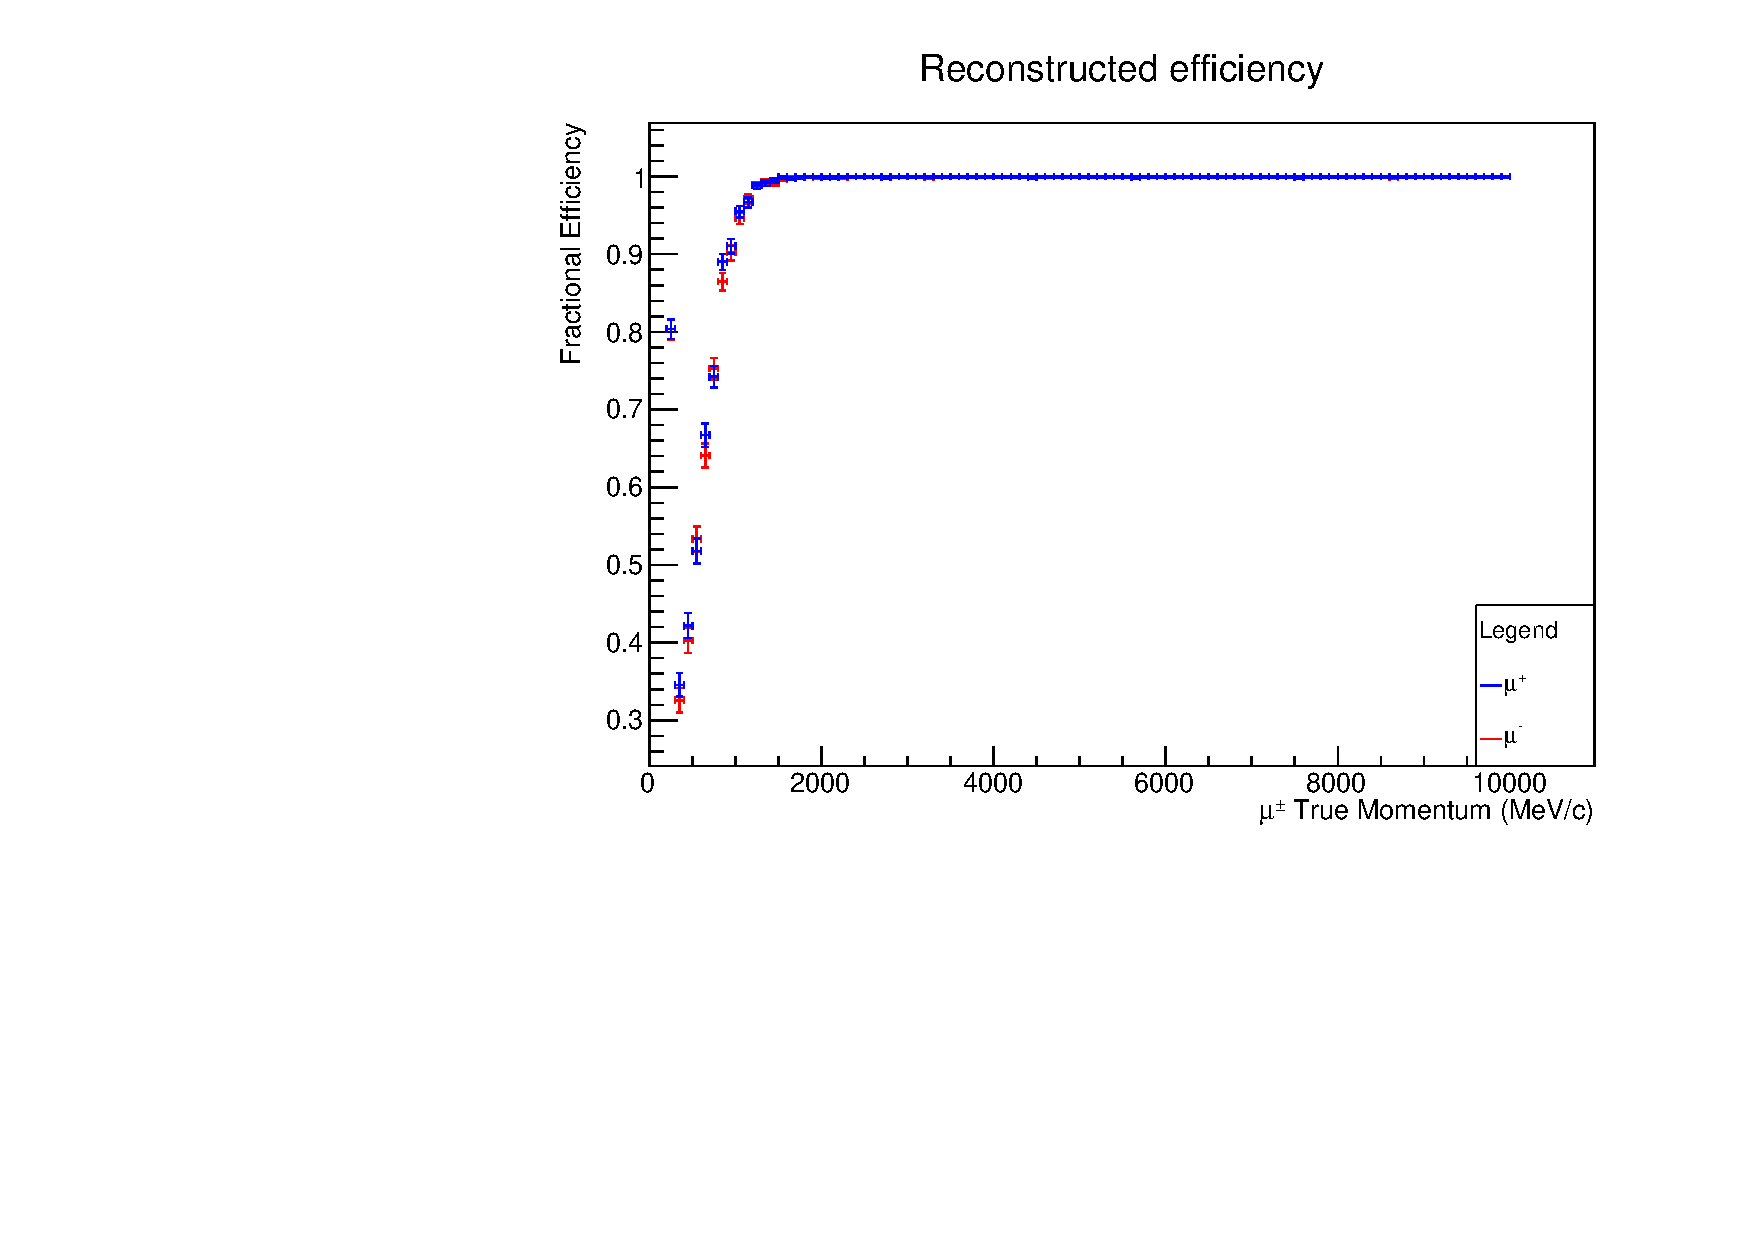
\includegraphics[width=0.6\textwidth]{FittedMuonBeam.pdf}
			
			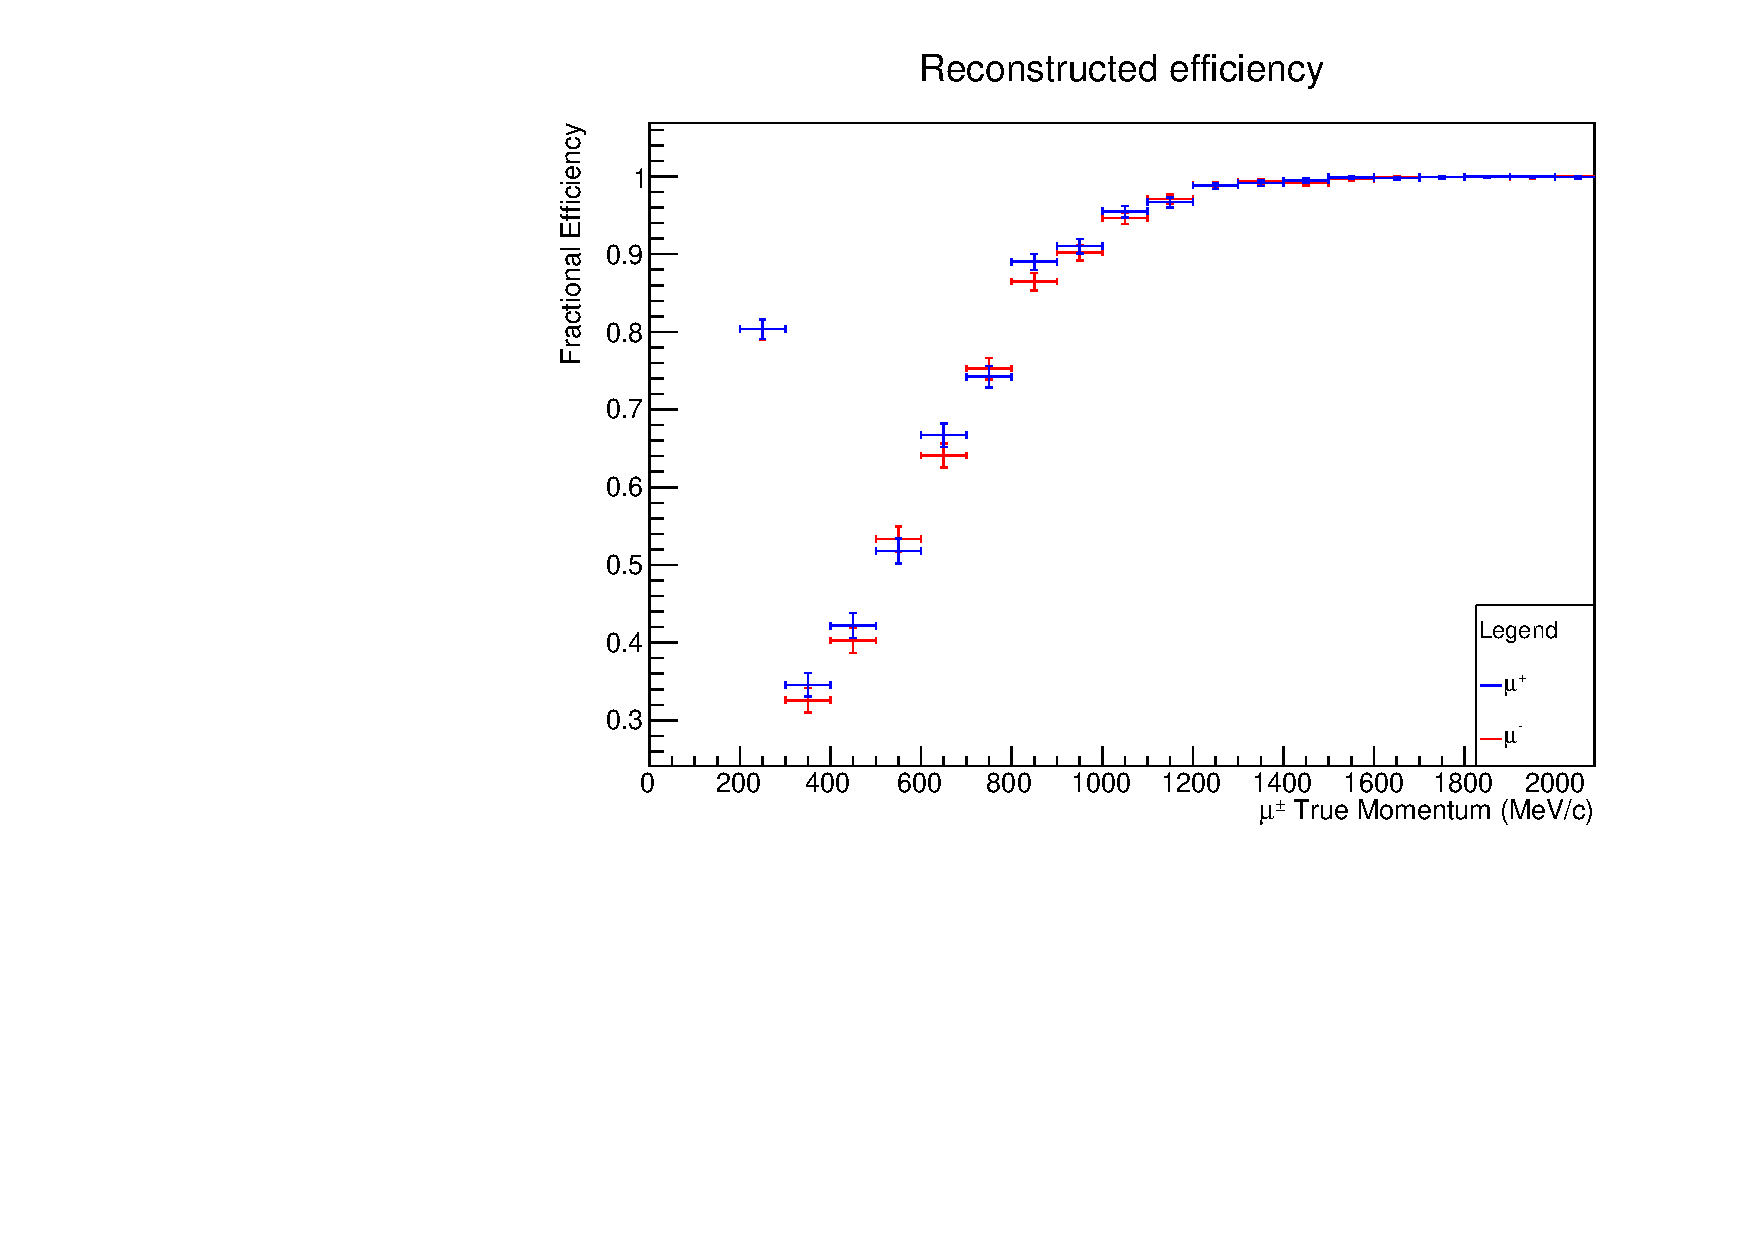
\includegraphics[width=0.6\textwidth]{FittedMuonBeamZoom.pdf}
		\end{figure}
	\end{column}%
	\begin{column}{.48\textwidth}
		\begin{figure}[h!]
			\centering
			%trim=l b r t
			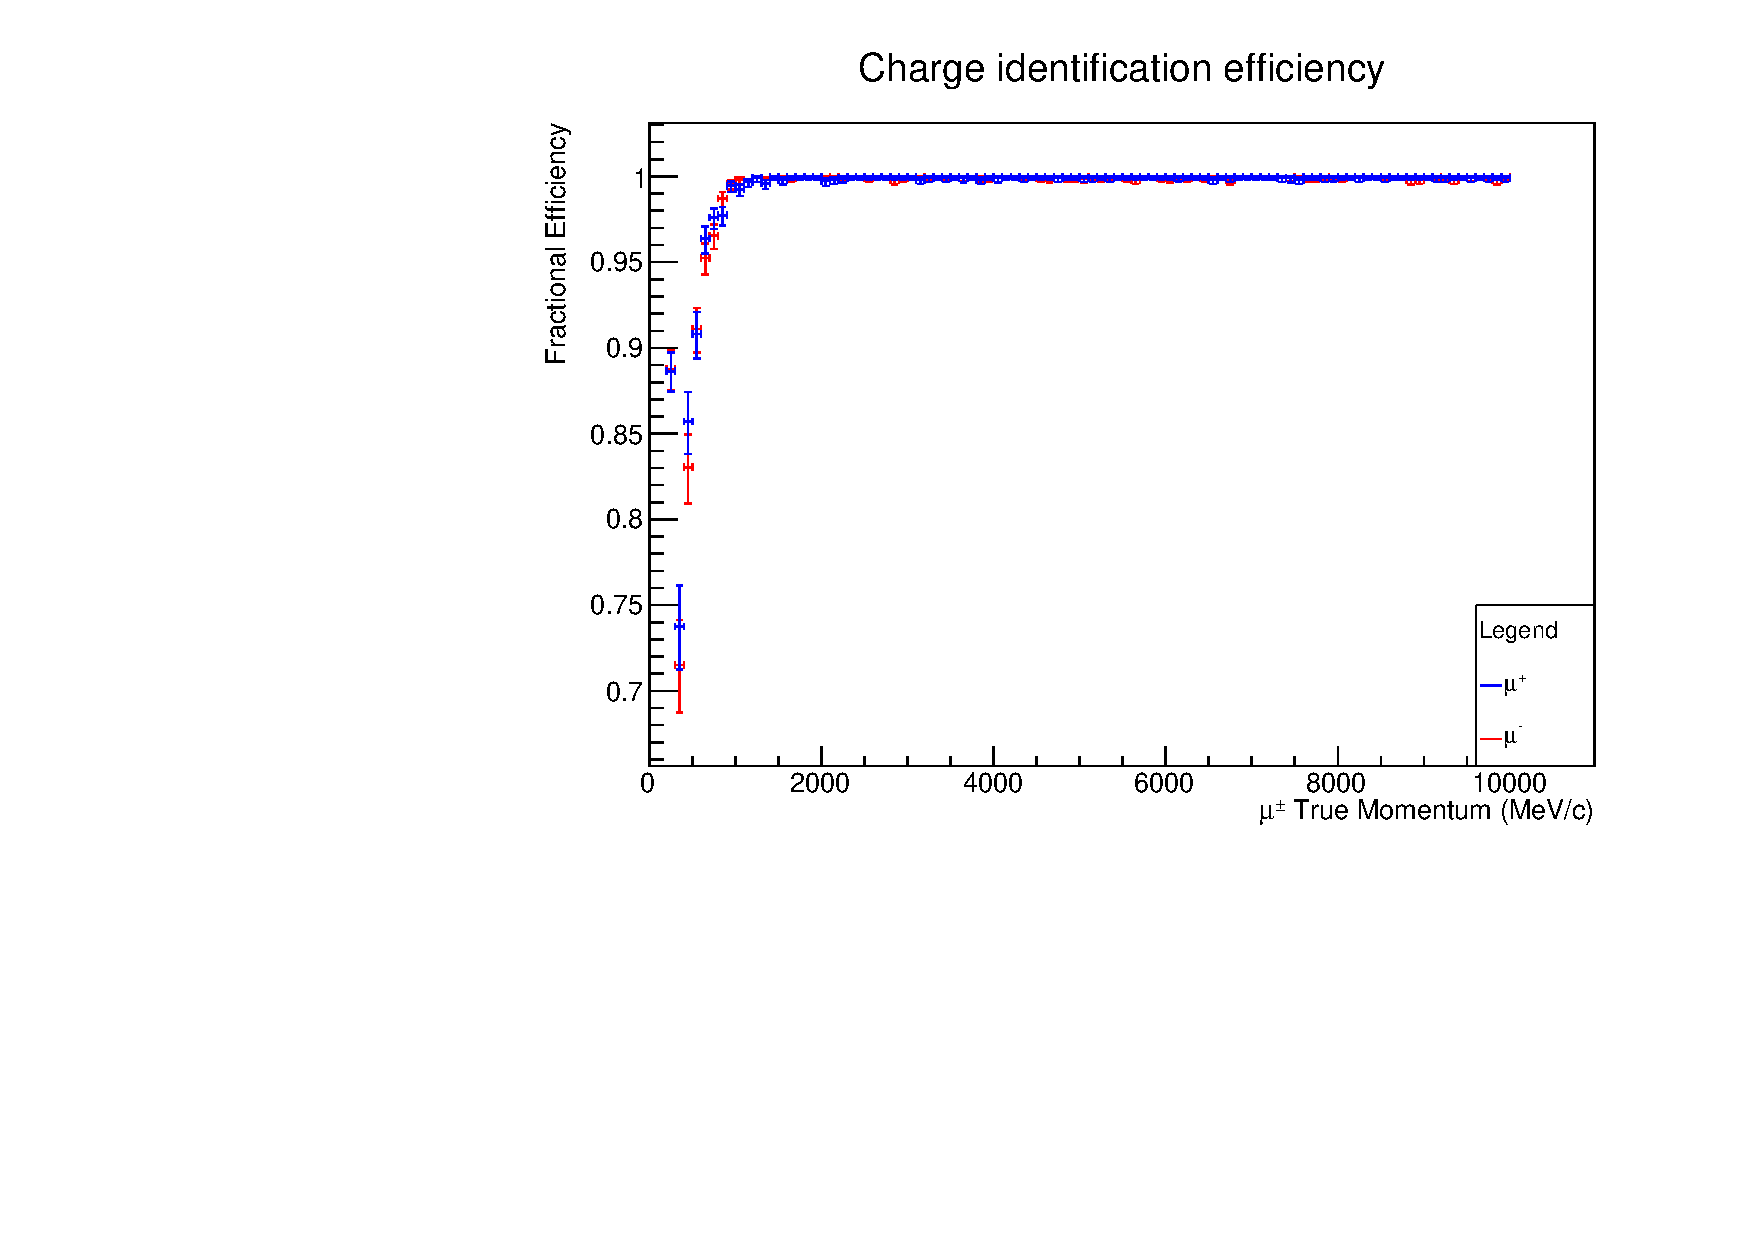
\includegraphics[width=0.6\textwidth]{ChargeIDMuonBeam.pdf}
			
				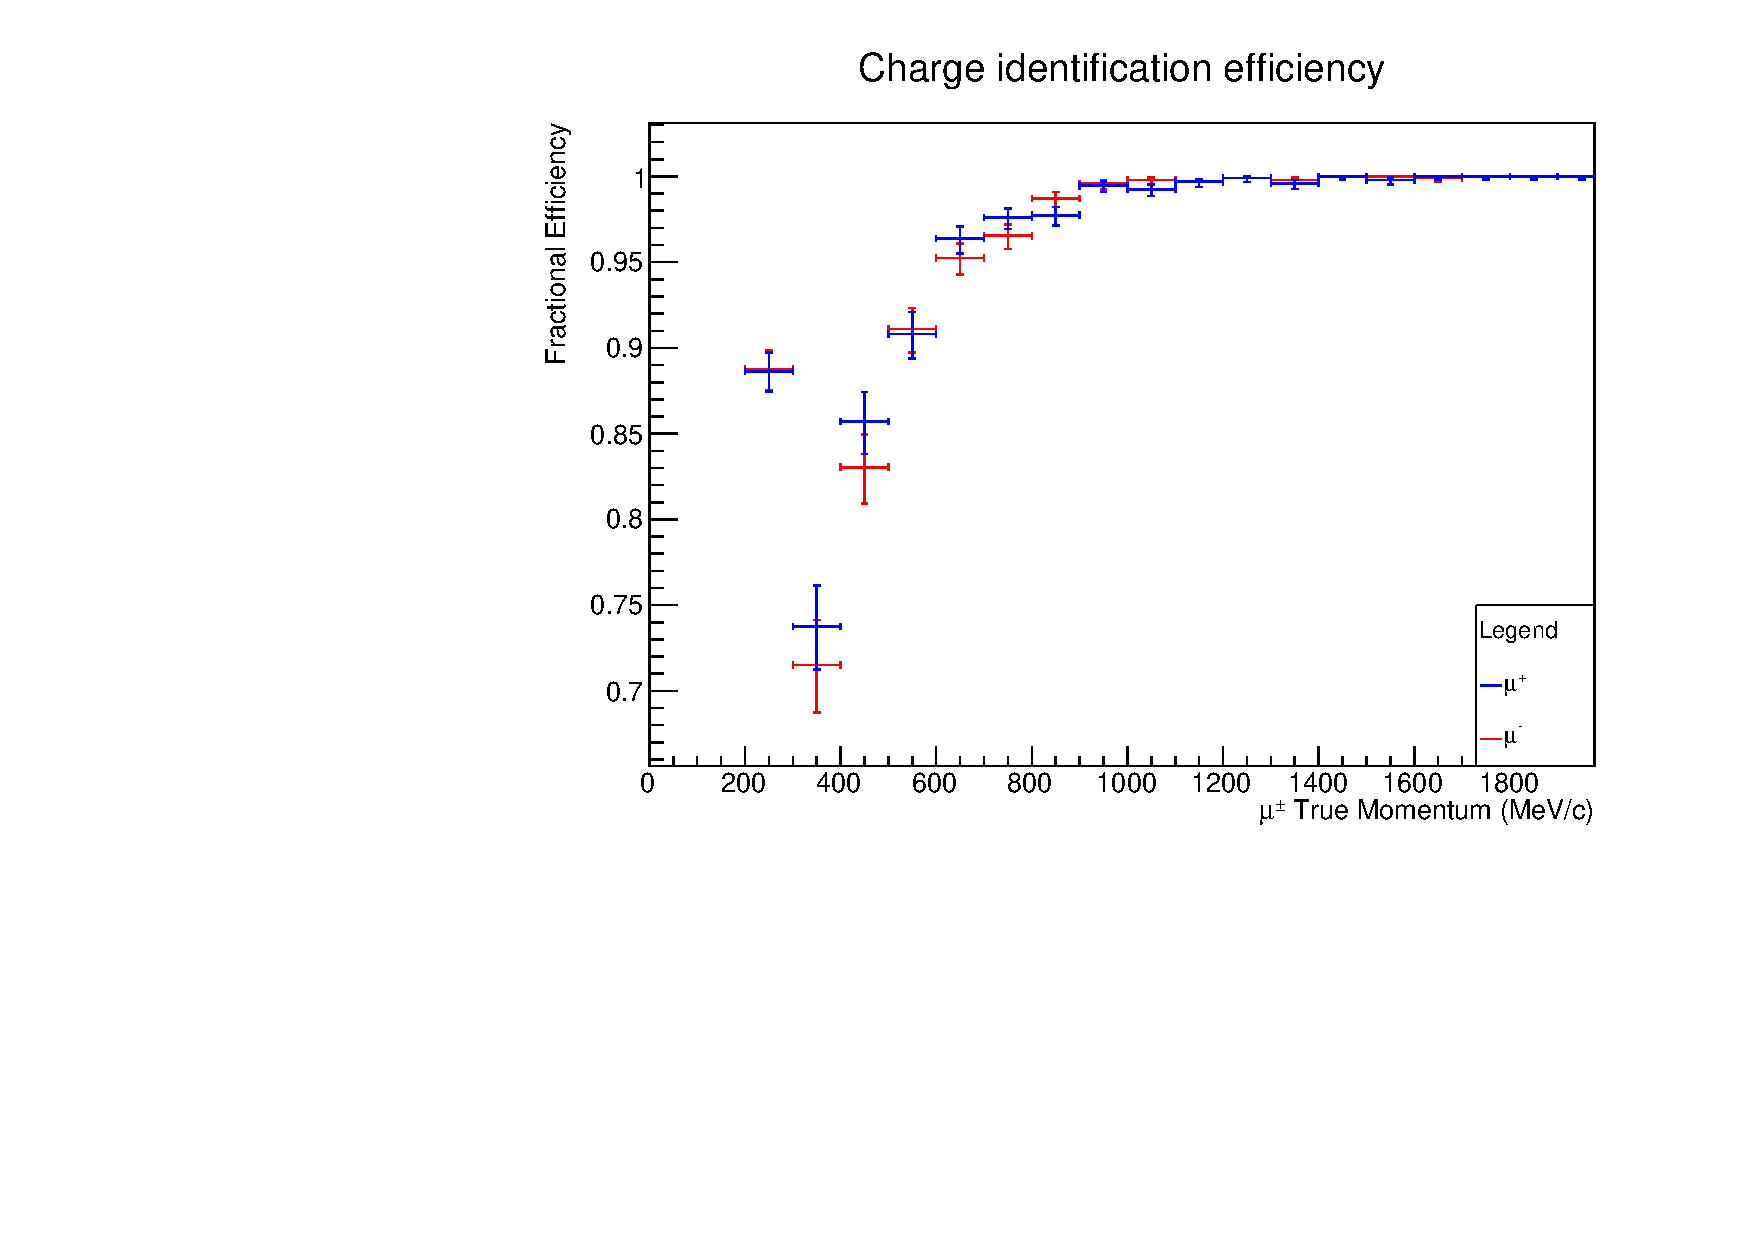
\includegraphics[width=0.6\textwidth]{ChargeIDMuonBeamZoom.pdf}
		\end{figure}
	\end{column}%
\end{columns}

\end{frame}

\begin{frame}{Monte Carlo events}

\begin{columns}[T] % align columns
	\begin{column}{.48\textwidth}
		
		\begin{figure}[h!]
			\centering
			%trim=l b r t
			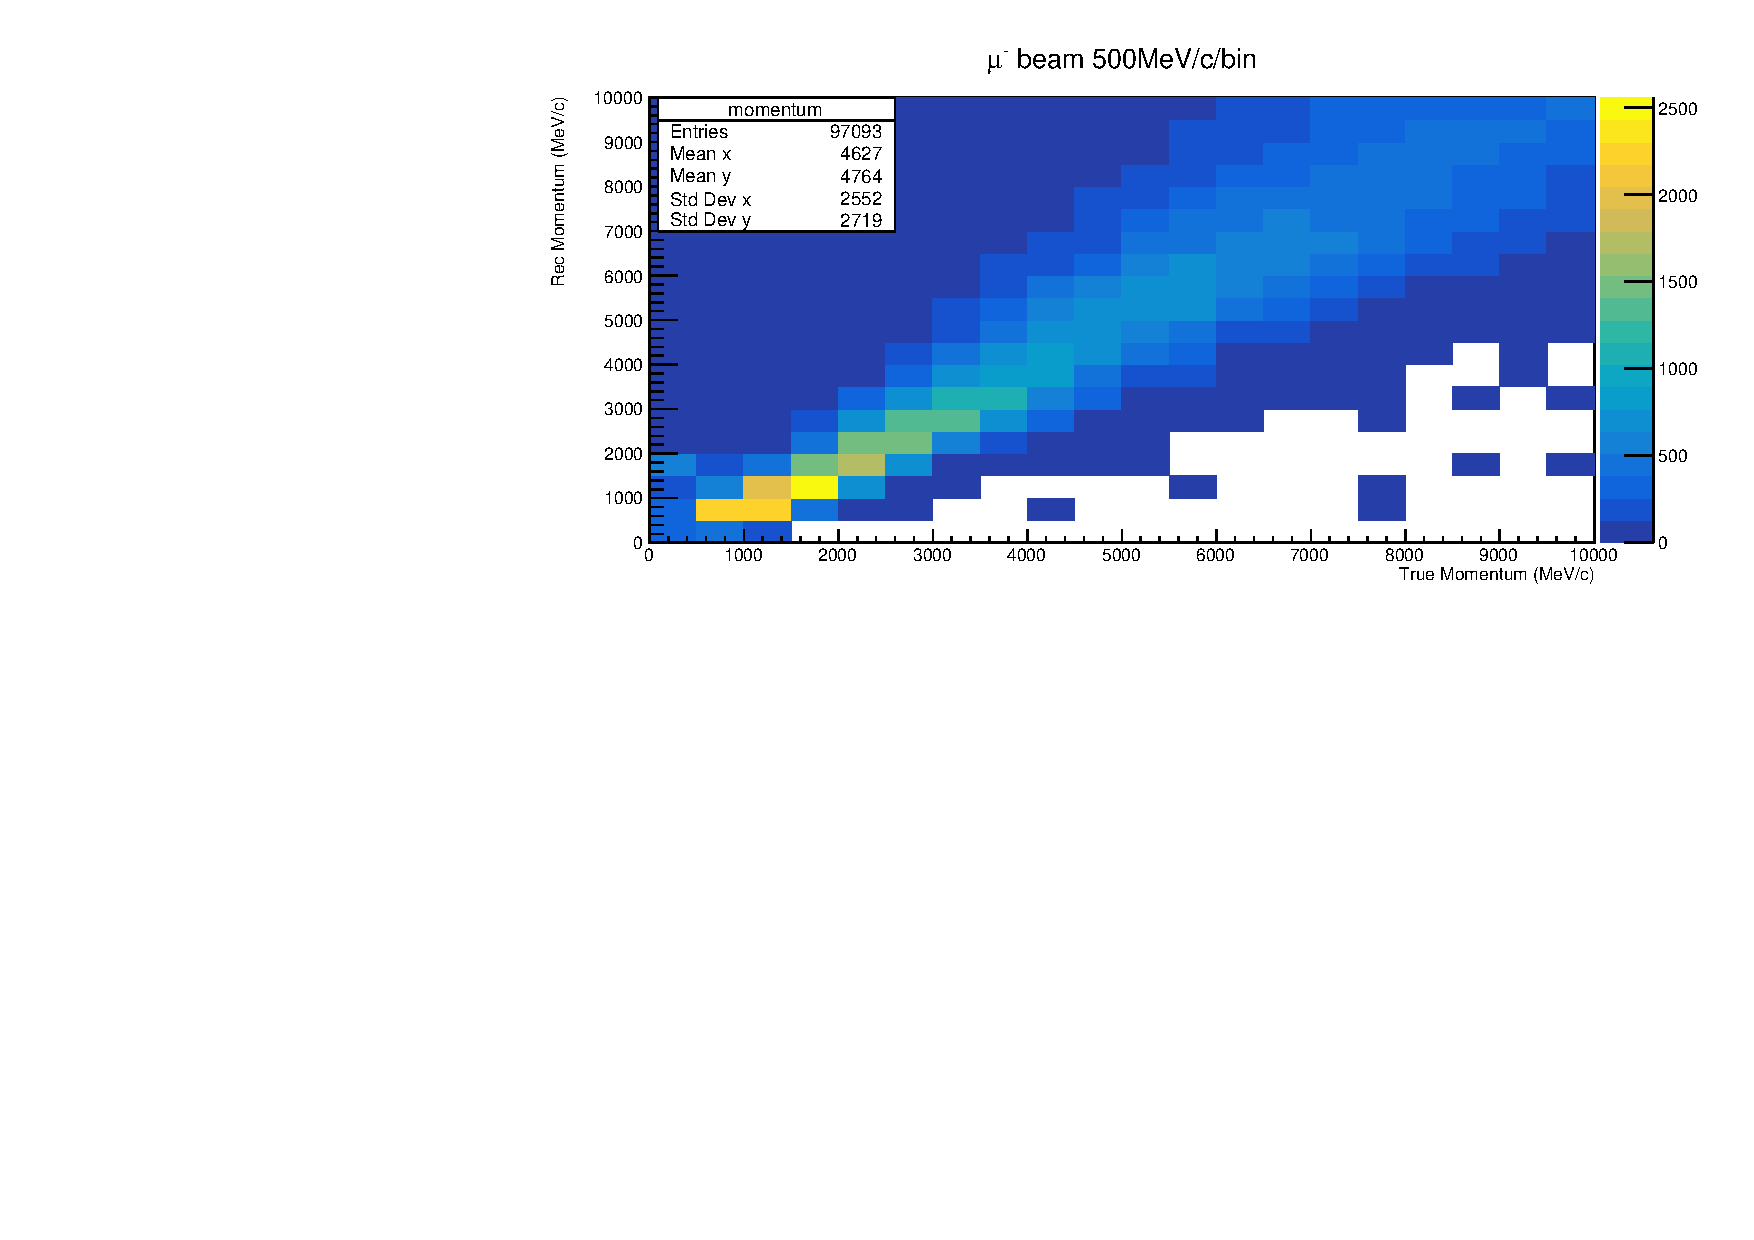
\includegraphics[width=\textwidth]{MomentumMuonBeam.pdf}
			
				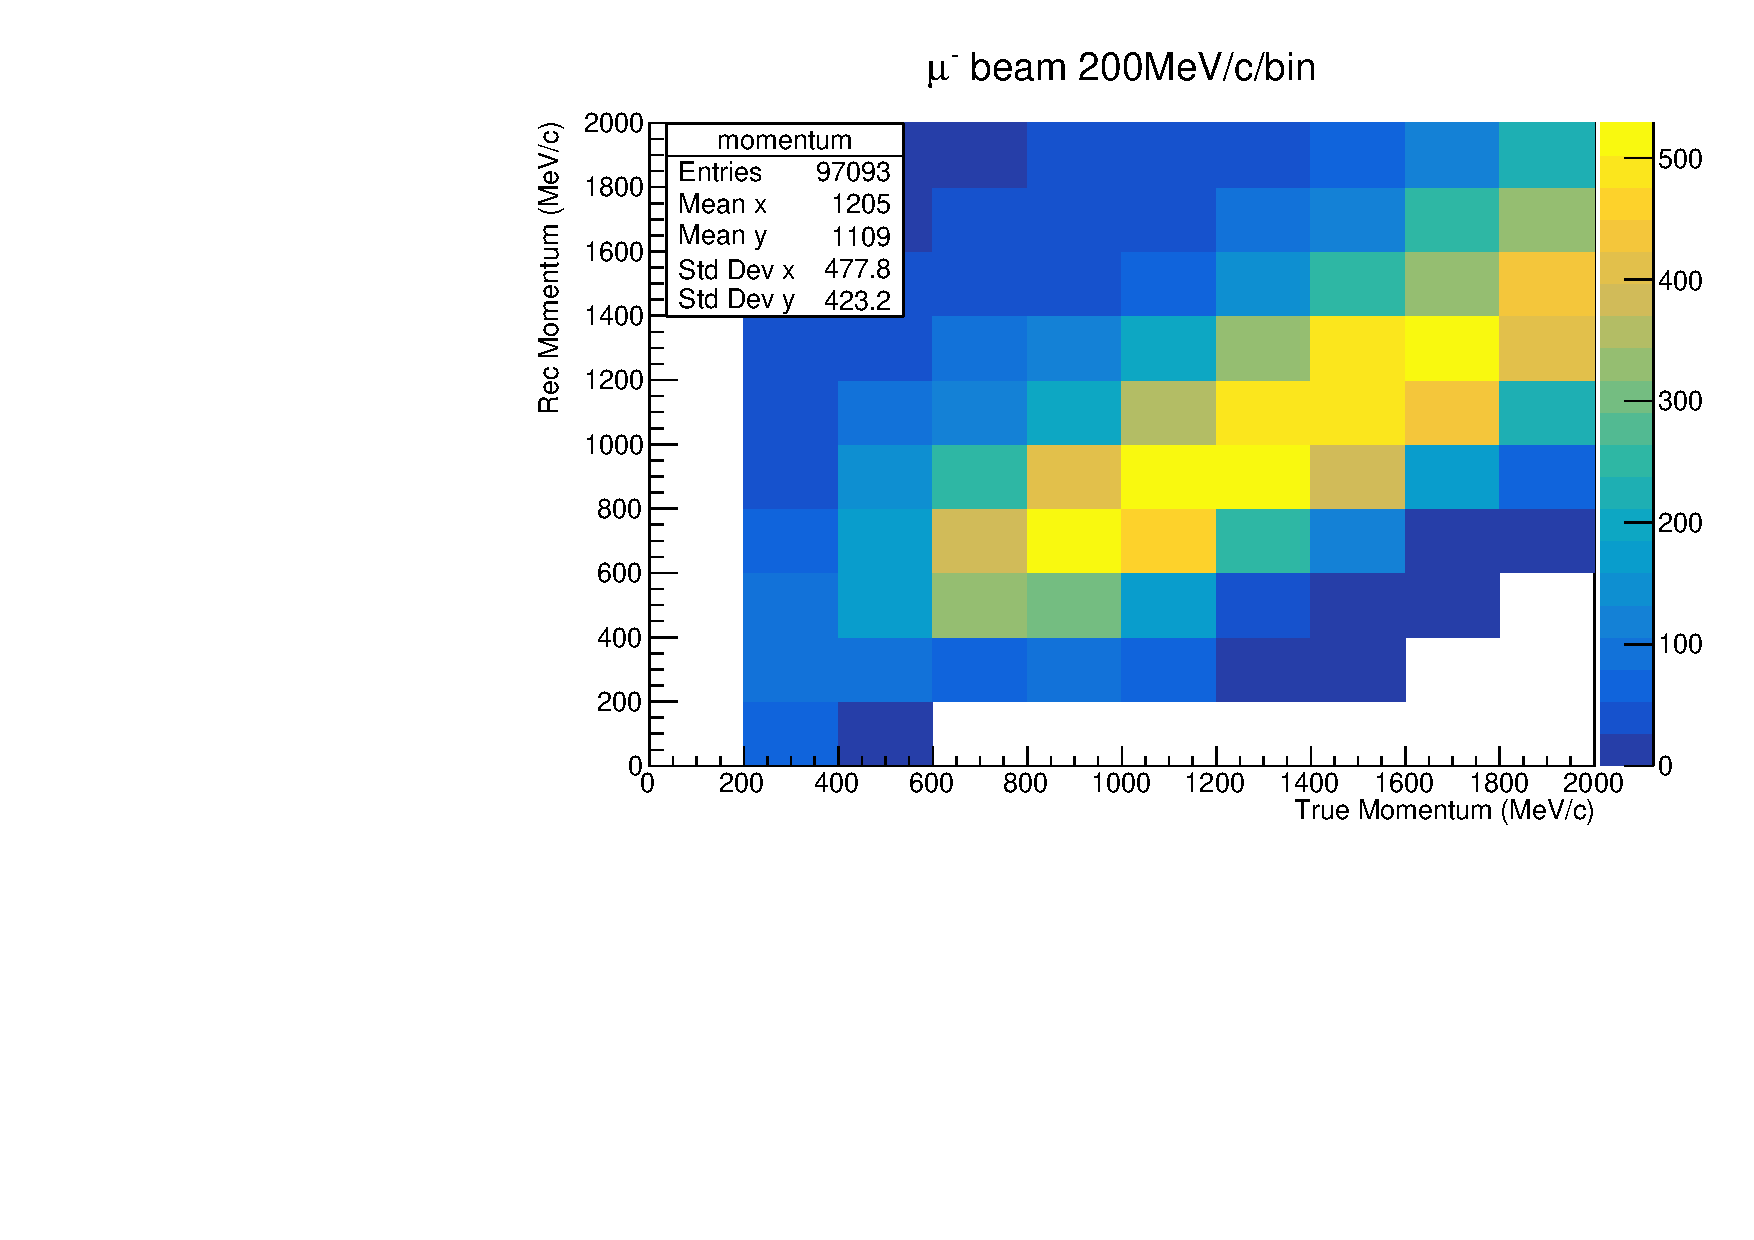
\includegraphics[width=\textwidth]{MomentumMuonBeamZoom.pdf}
		\end{figure}
	\end{column}%
	\begin{column}{.48\textwidth}
		\begin{figure}[h!]
			\centering
			%trim=l b r t
			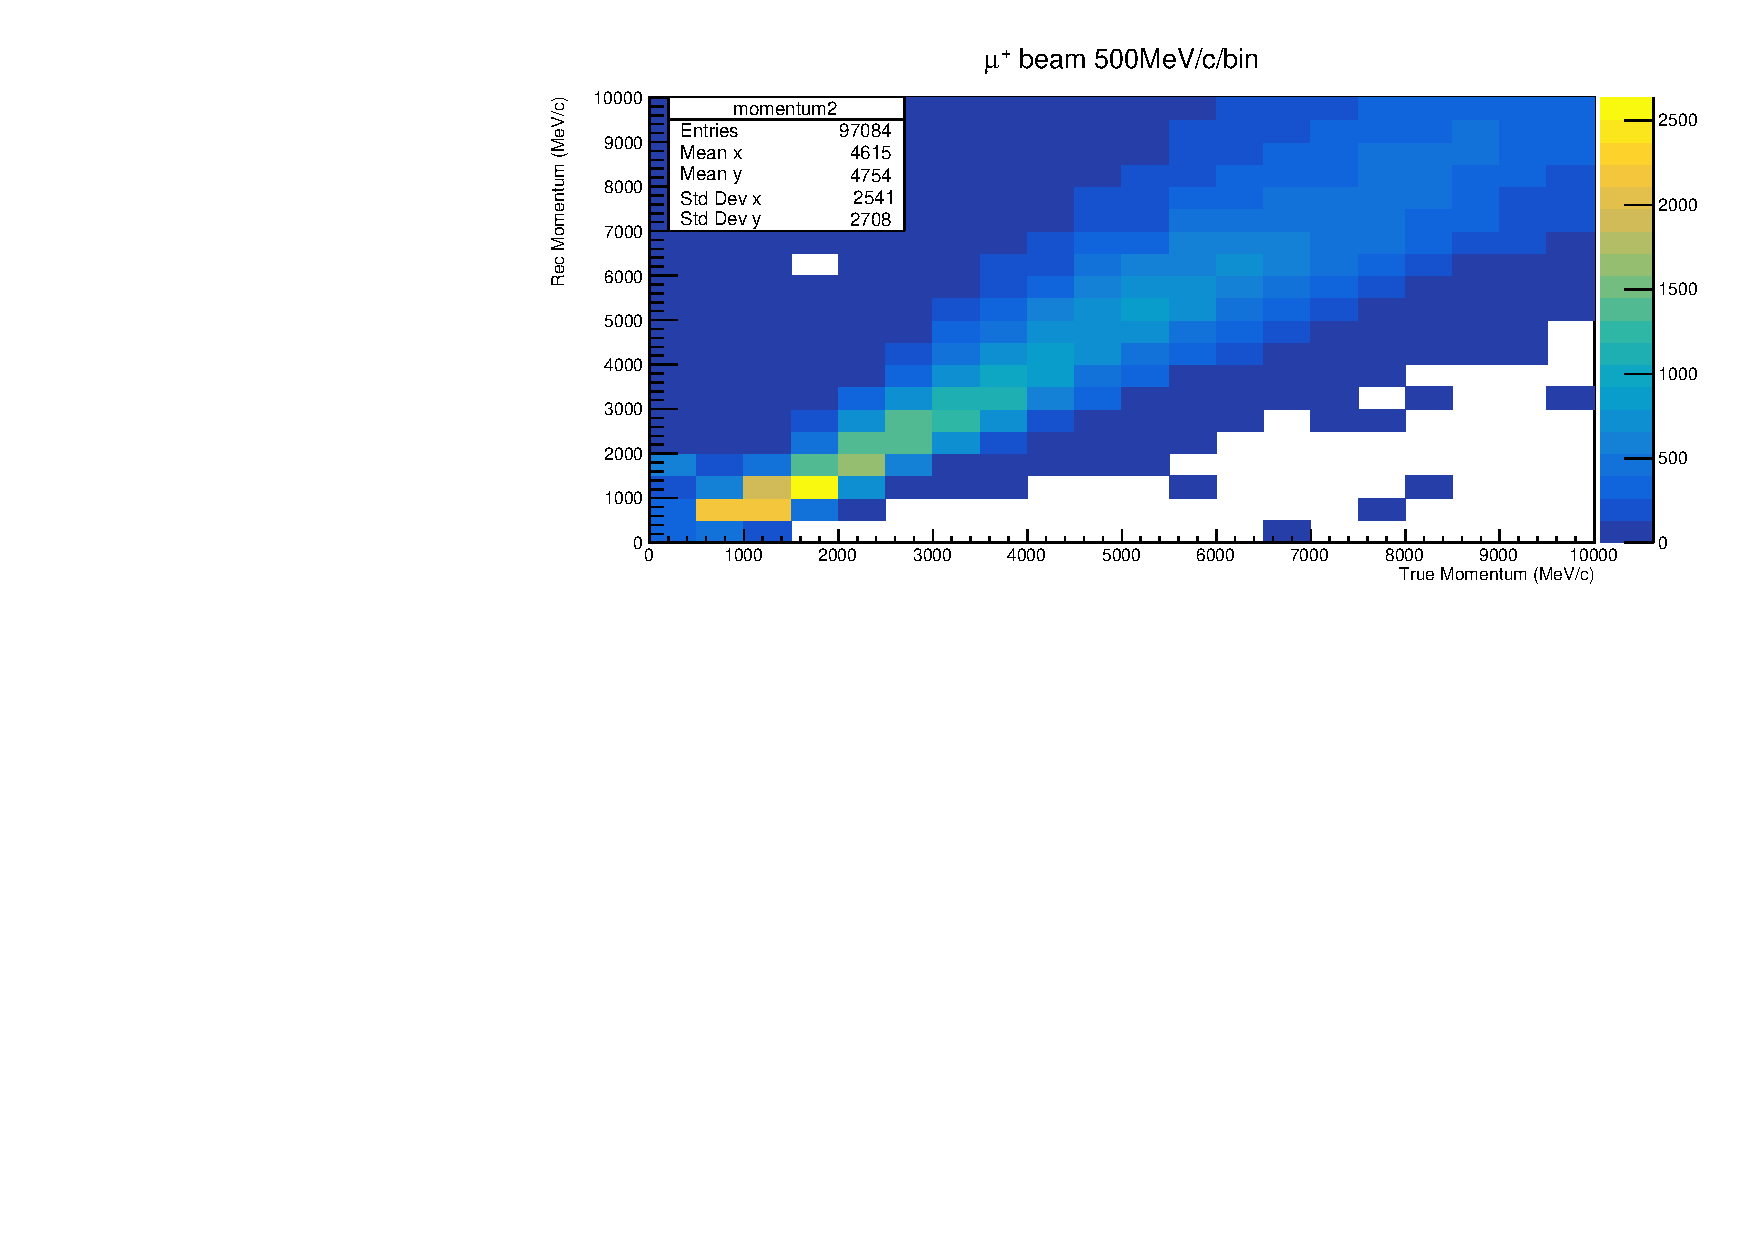
\includegraphics[width=\textwidth]{MomentumAntiMuonBeam.pdf}
			
				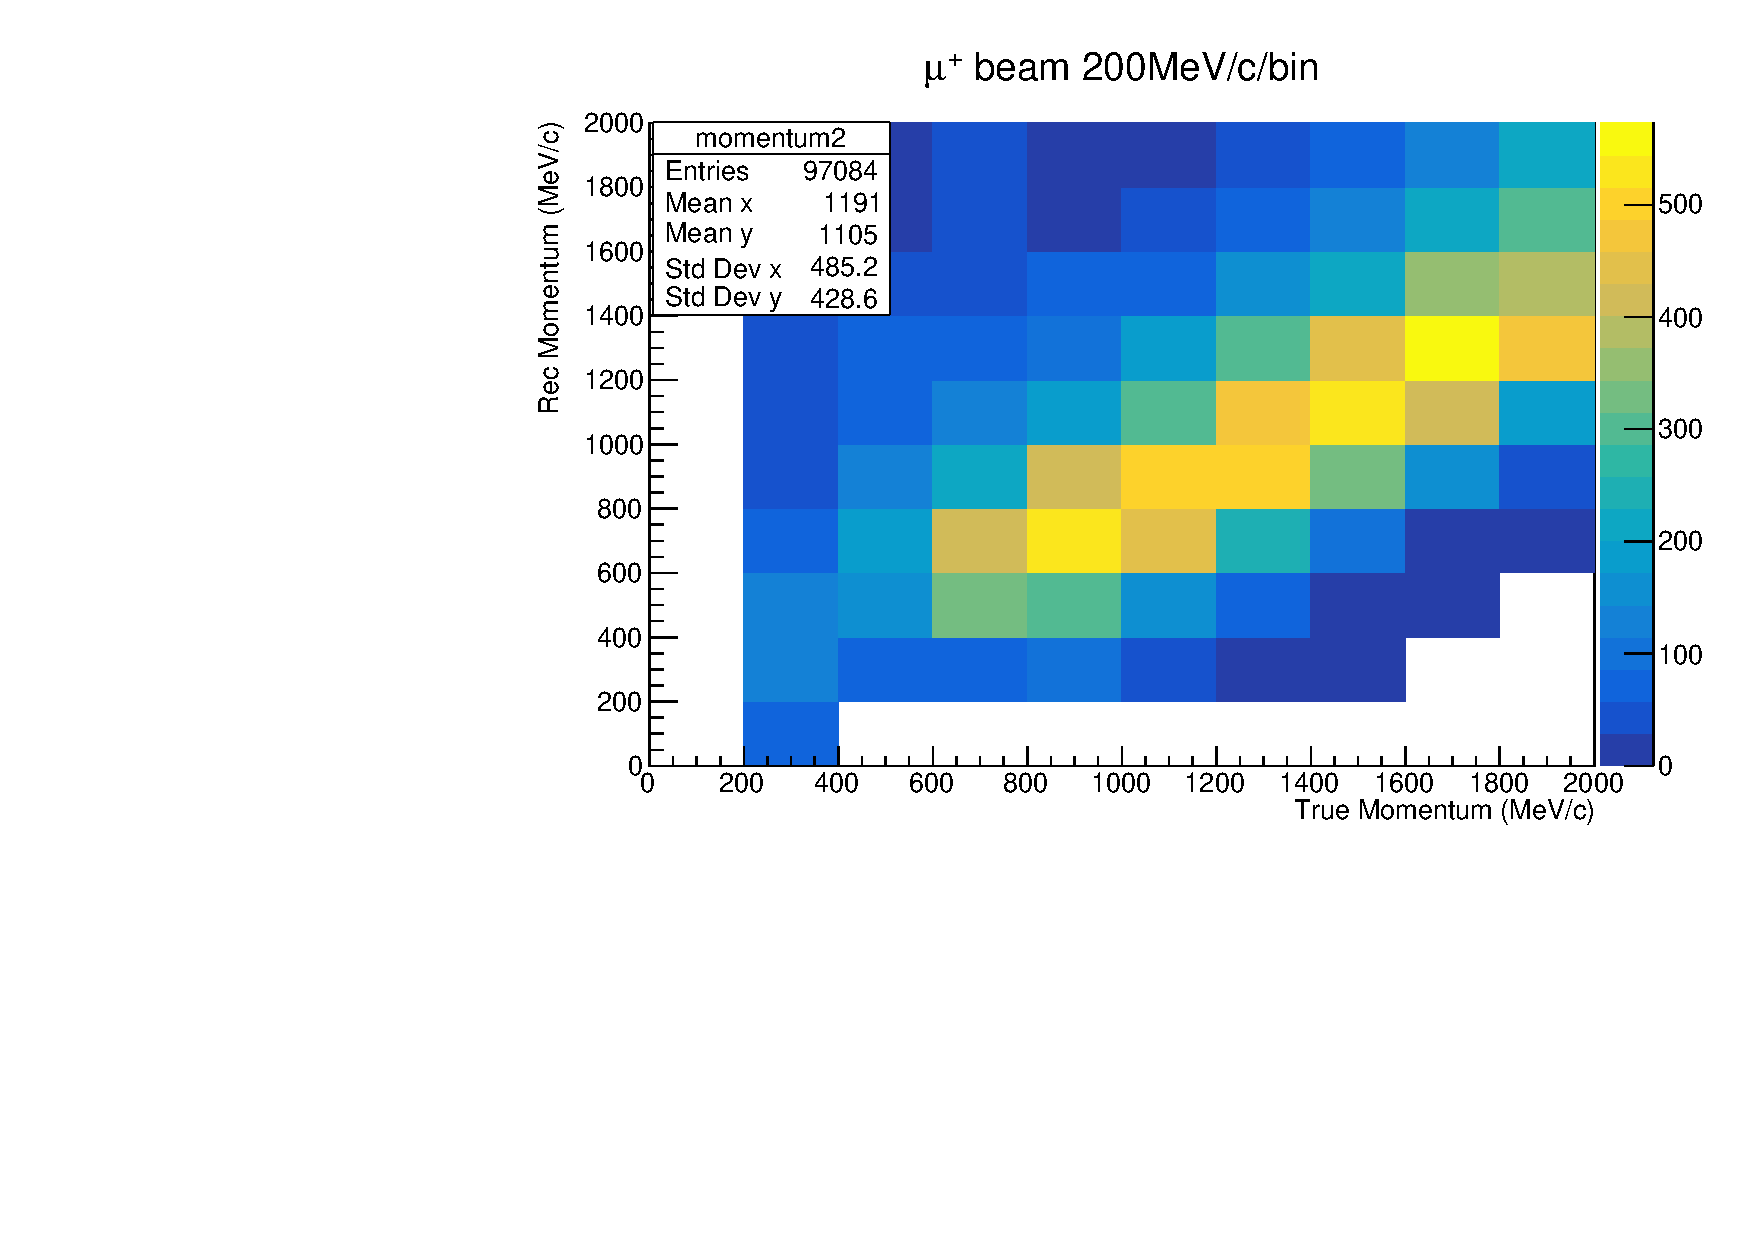
\includegraphics[width=\textwidth]{MomentumAntiMuonBeamZoom.pdf}
		\end{figure}
	\end{column}%
\end{columns}

\end{frame}

\begin{frame}{Monte Carlo events}
		\begin{figure}[h!]
	\centering
	%trim=l b r t
	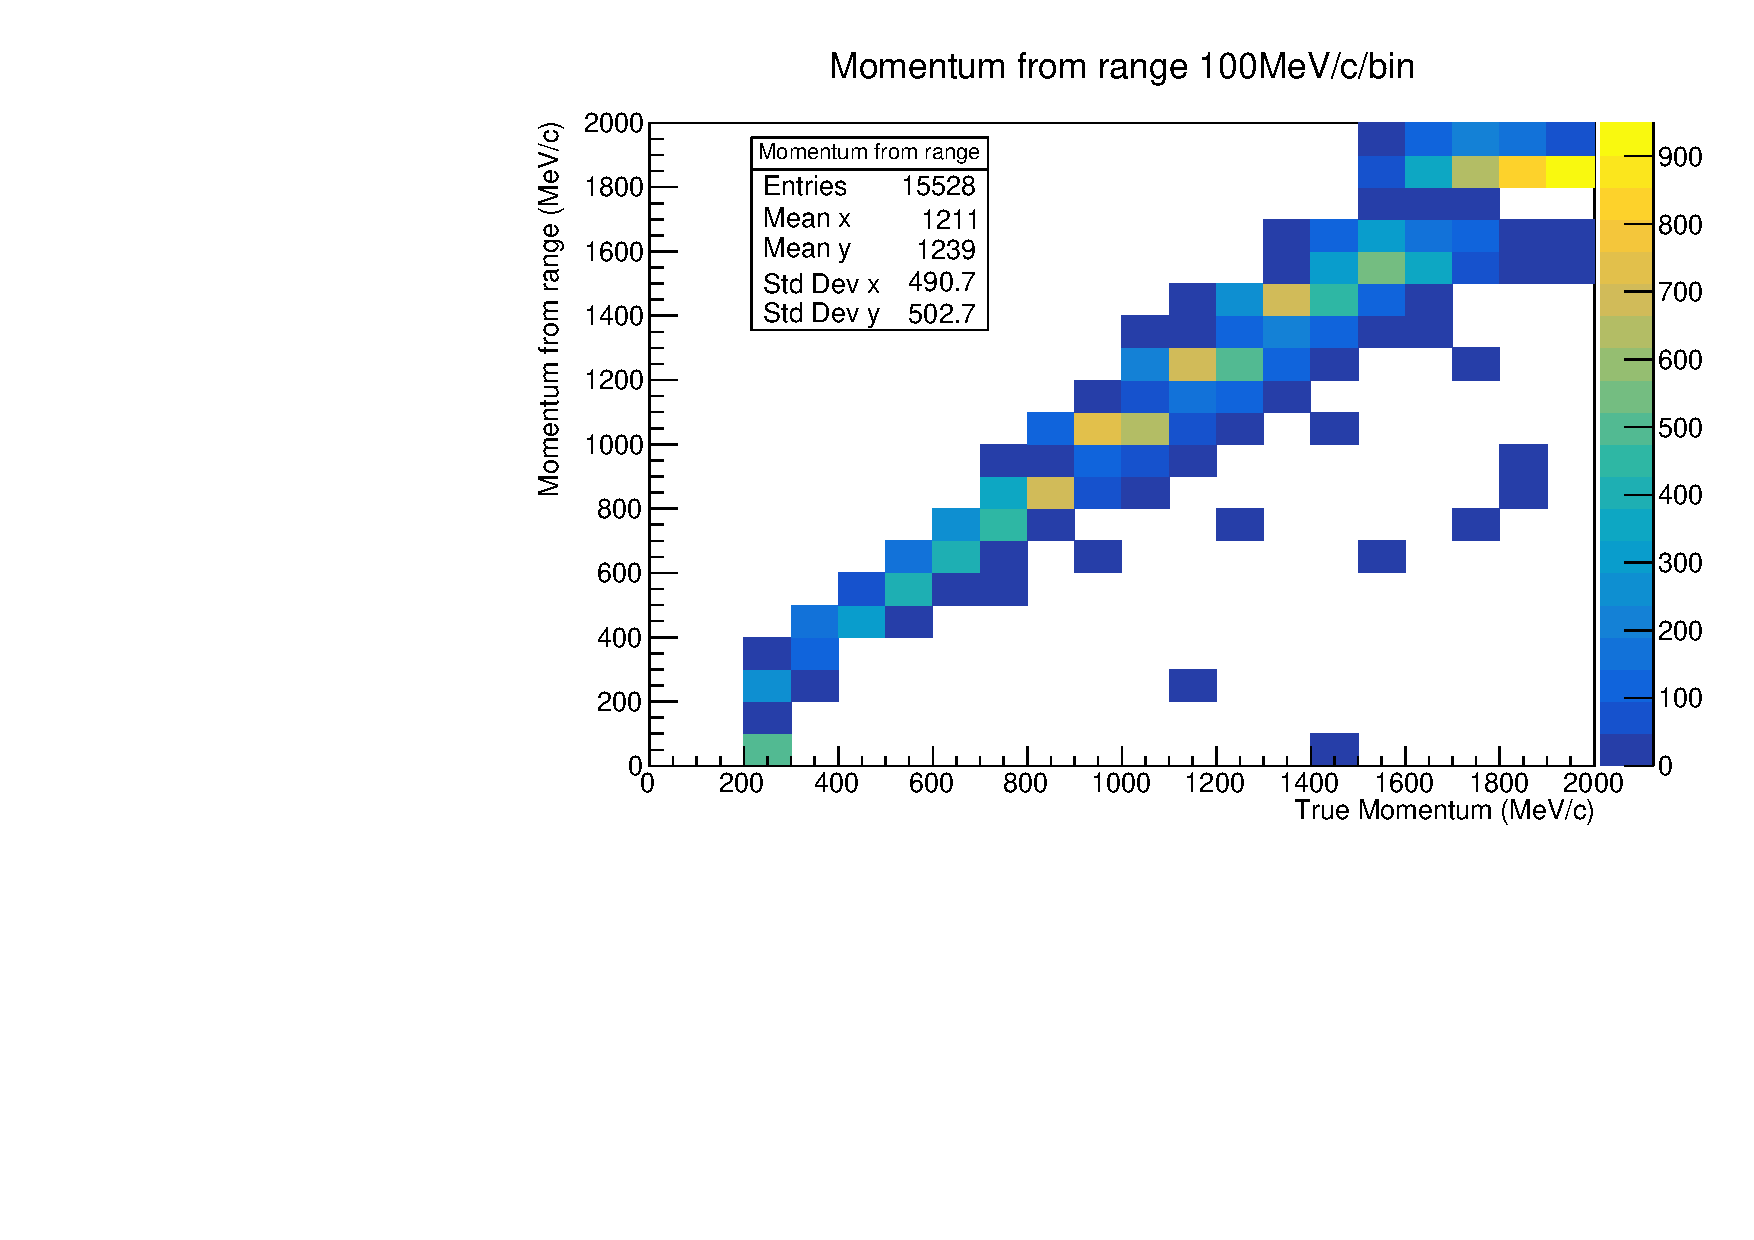
\includegraphics[width=\textwidth]{MomentumRangeMuonBeam.pdf}
\end{figure}
\end{frame}

\begin{frame}{From the nuSTORM beam}
\begin{block}{}
	\begin{tiny}
		\begin{itemize}
\item Interactions in MIND with NuStorm beam.
		\end{itemize}
	\end{tiny}
\end{block}
\begin{columns}[T] % align columns
	\begin{column}{.48\textwidth}
		
		\begin{figure}[h!]
			\centering
			%trim=l b r t
			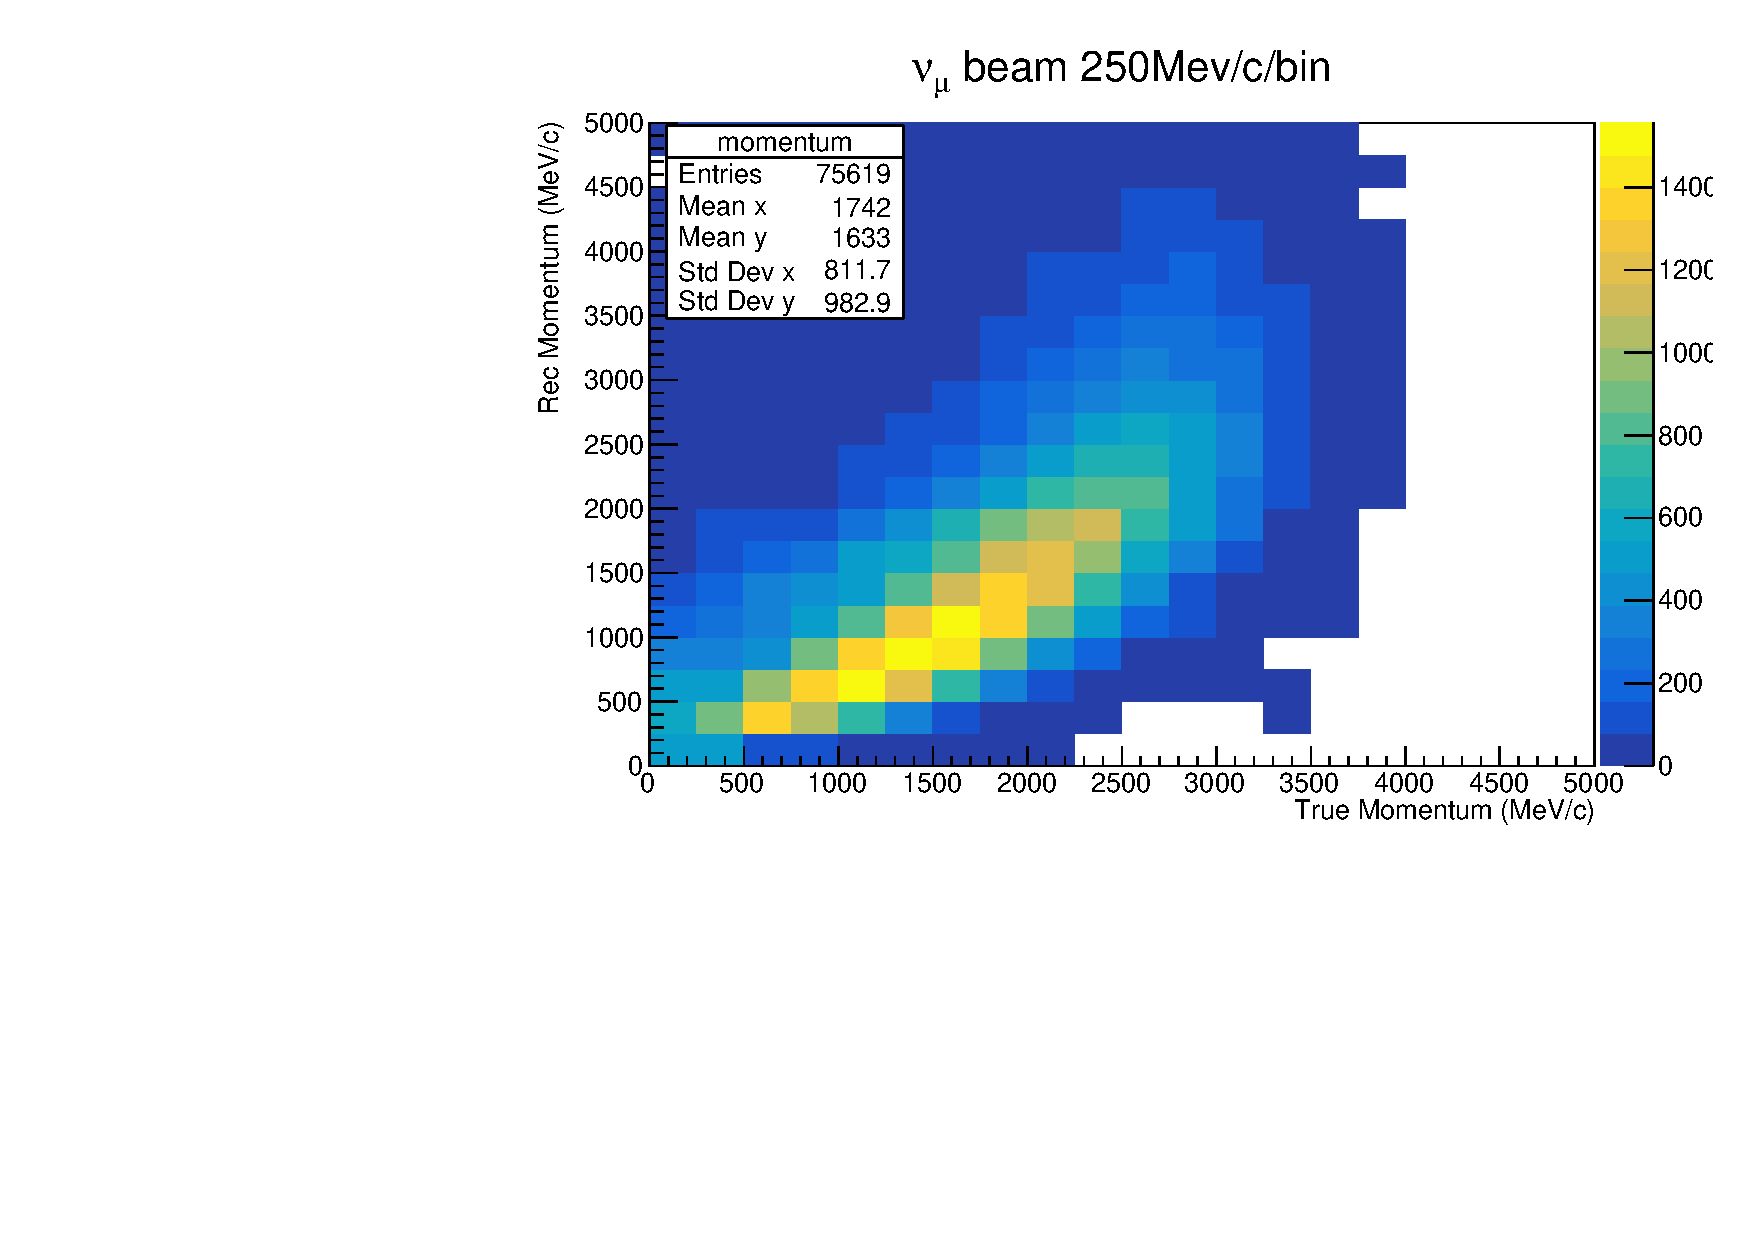
\includegraphics[width=\textwidth]{NuStorm/MomentumNeutrinoBeamMIND.pdf}
		\end{figure}
	\end{column}%
	\begin{column}{.48\textwidth}
		\begin{figure}[h!]
			\centering
			%trim=l b r t
			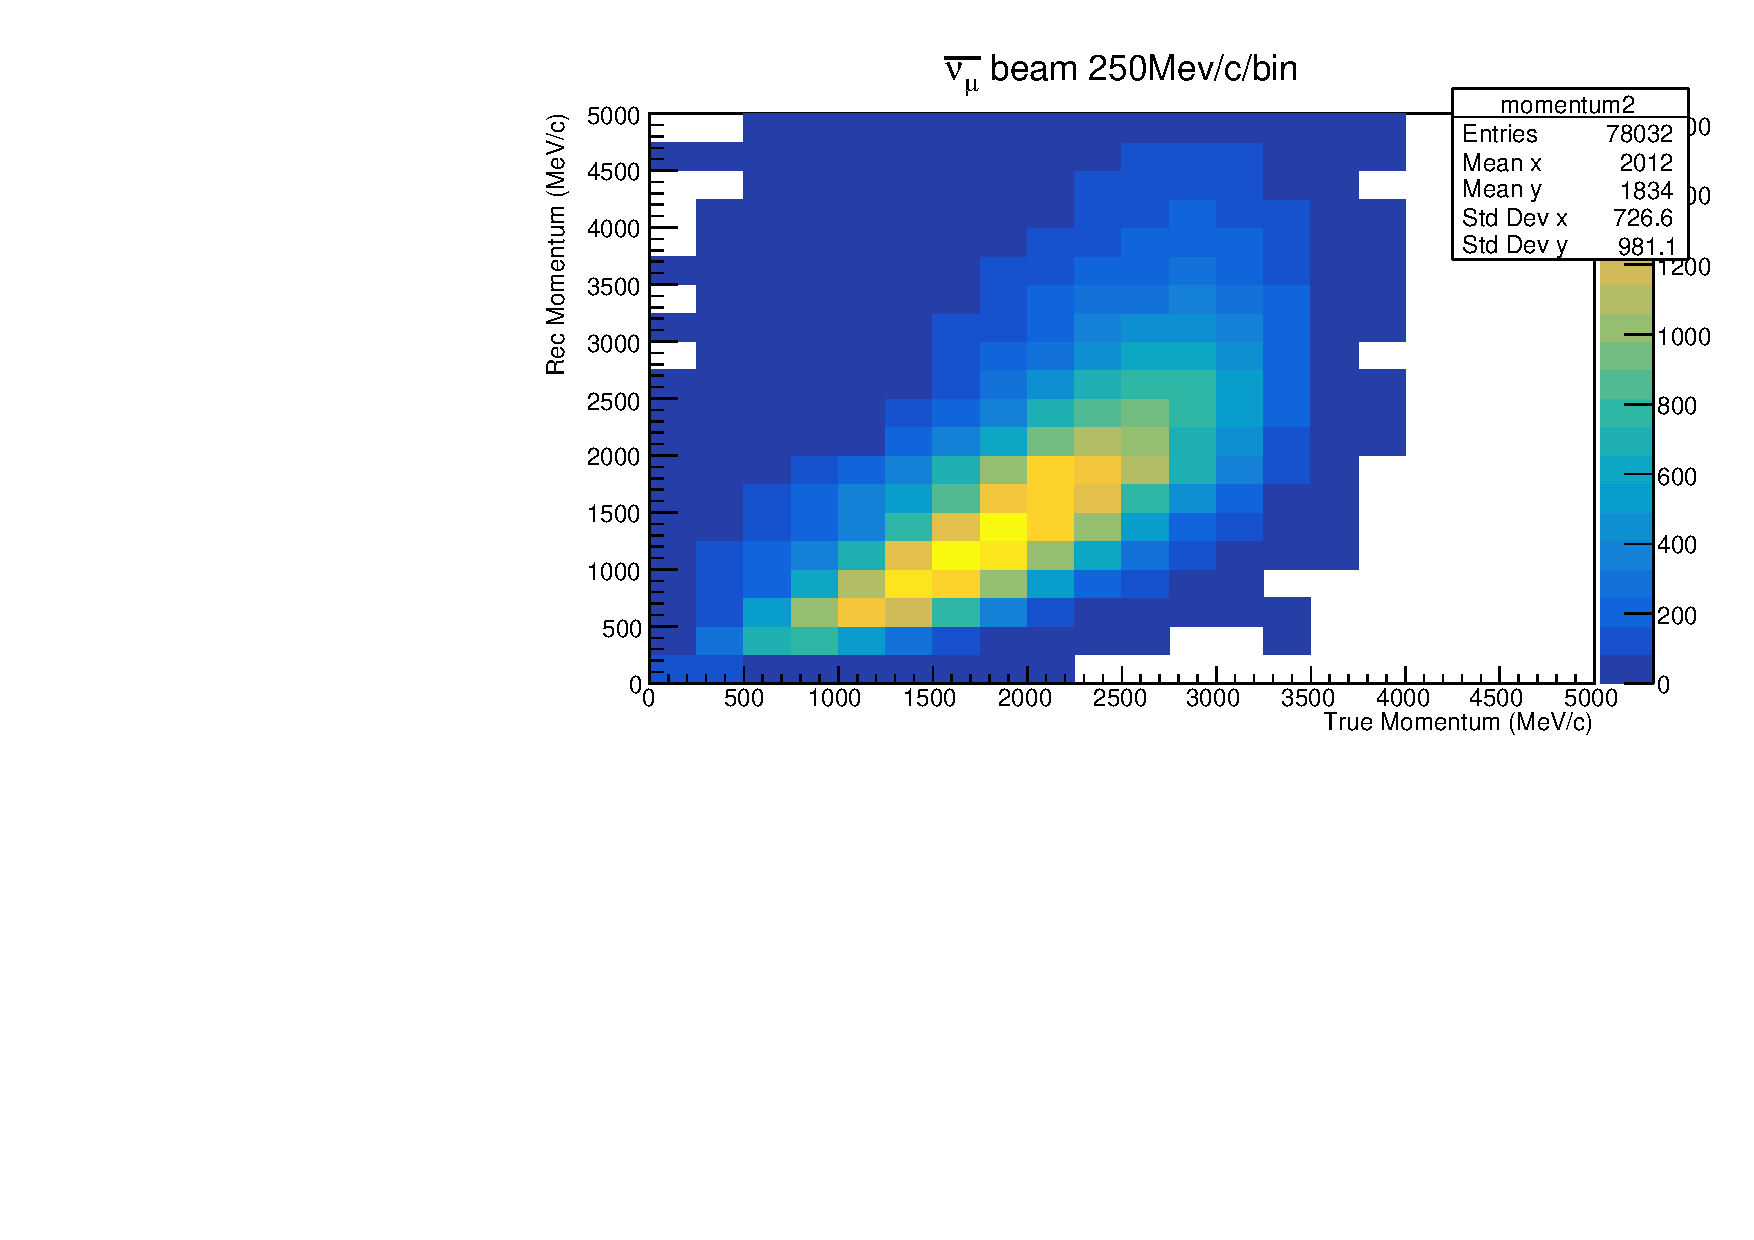
\includegraphics[width=\textwidth]{NuStorm/MomentumAntiNeutrinoBeamMIND.pdf}
		\end{figure}
	\end{column}%
\end{columns}
\end{frame}

\begin{frame}{From the nuSTORM beam}
\begin{block}{}
	\begin{tiny}
		\begin{itemize}
			\item Interactions in MIND with NuStorm beam.
		\end{itemize}
	\end{tiny}
\end{block}
\begin{columns}[T] % align columns
	\begin{column}{.48\textwidth}
		
		\begin{figure}[h!]
			\centering
			%trim=l b r t
			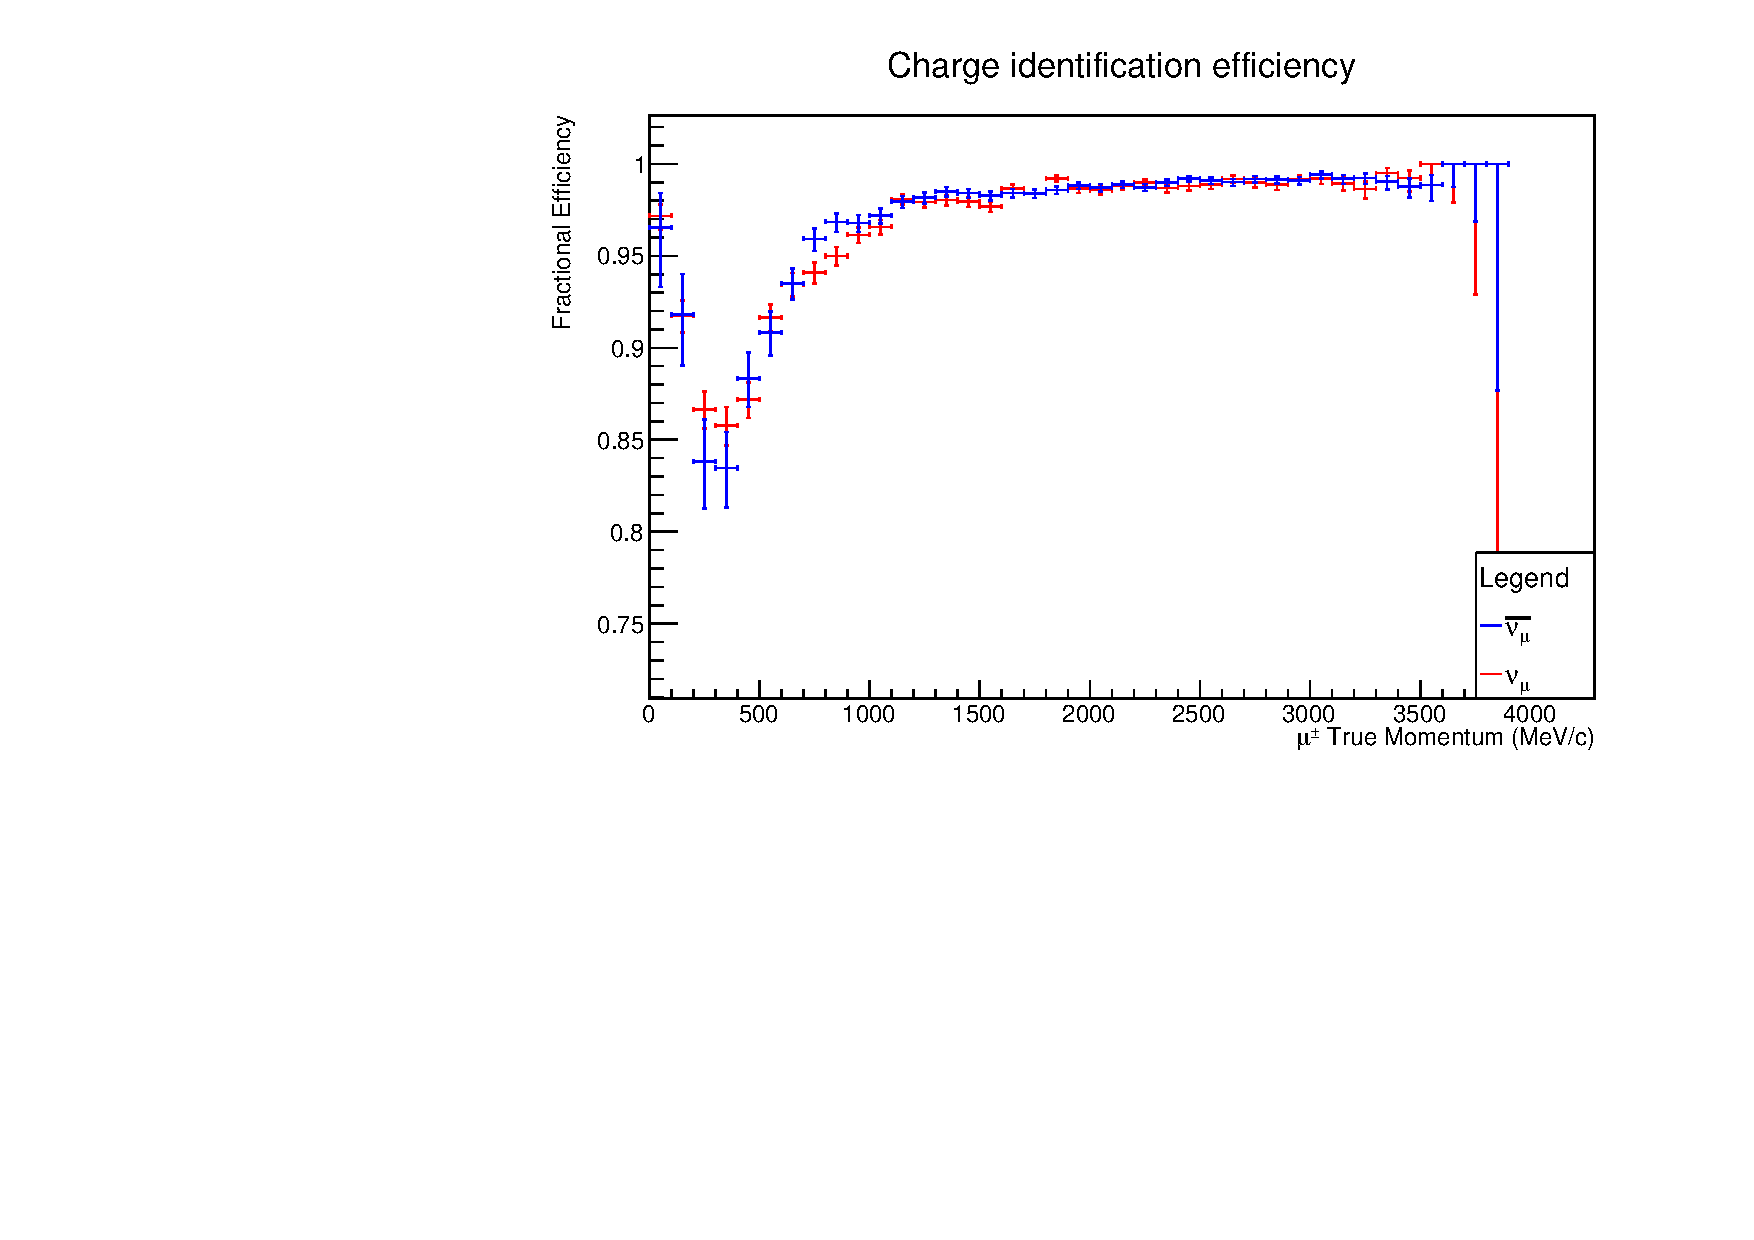
\includegraphics[width=\textwidth]{NuStorm/ChargeIDNeutrinoBeamMIND.pdf}
		\end{figure}
	\end{column}%
	\begin{column}{.48\textwidth}
		\begin{figure}[h!]
			\centering
			%trim=l b r t
			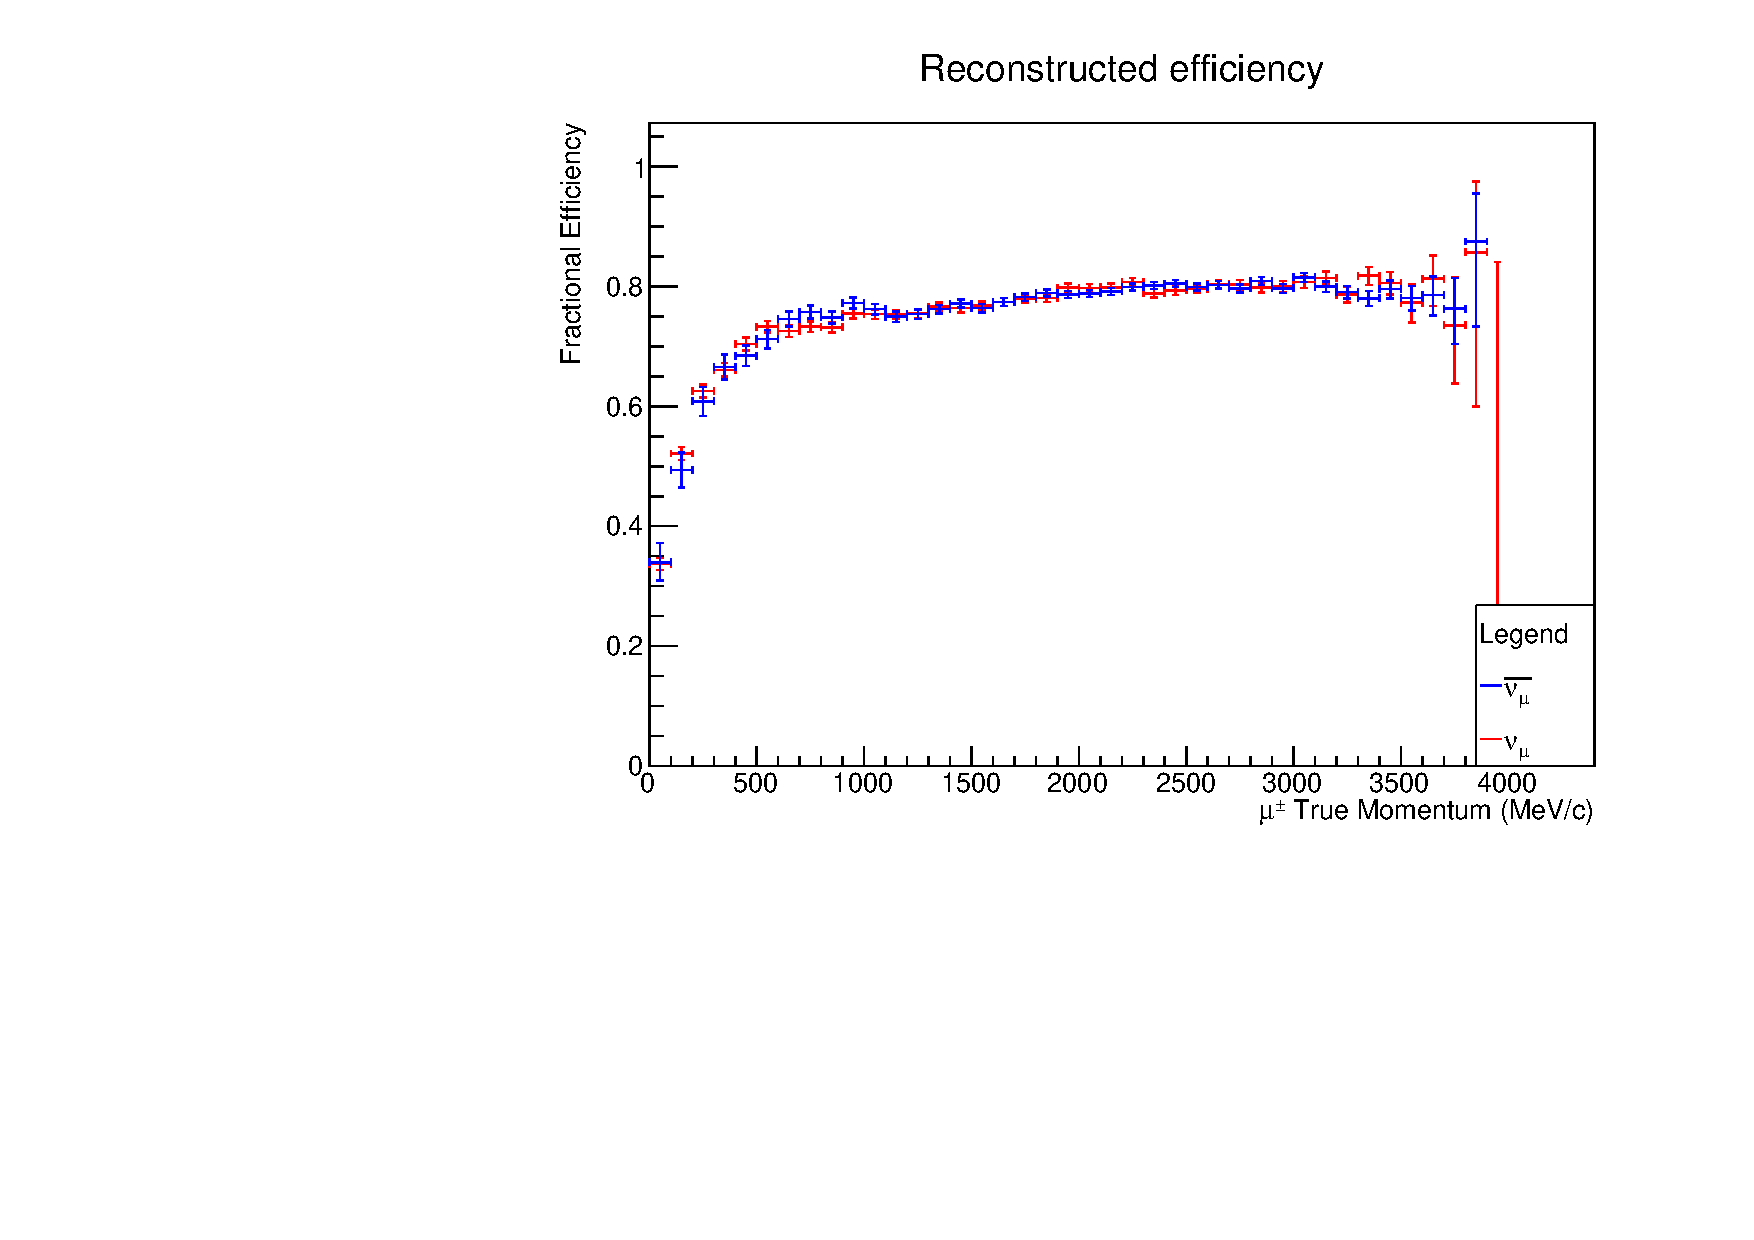
\includegraphics[width=\textwidth]{NuStorm/FittedNeutrinoBeamMIND.pdf}
		\end{figure}
	\end{column}%
\end{columns}
\end{frame}

\begin{frame}{From the nuSTORM beam}
\begin{block}{}
	\begin{tiny}
		\begin{itemize}
			\item Interactions in TASD with NuStorm beam.
		\end{itemize}
	\end{tiny}
\end{block}
\begin{columns}[T] % align columns
	\begin{column}{.48\textwidth}
		
		\begin{figure}[h!]
			\centering
			%trim=l b r t
			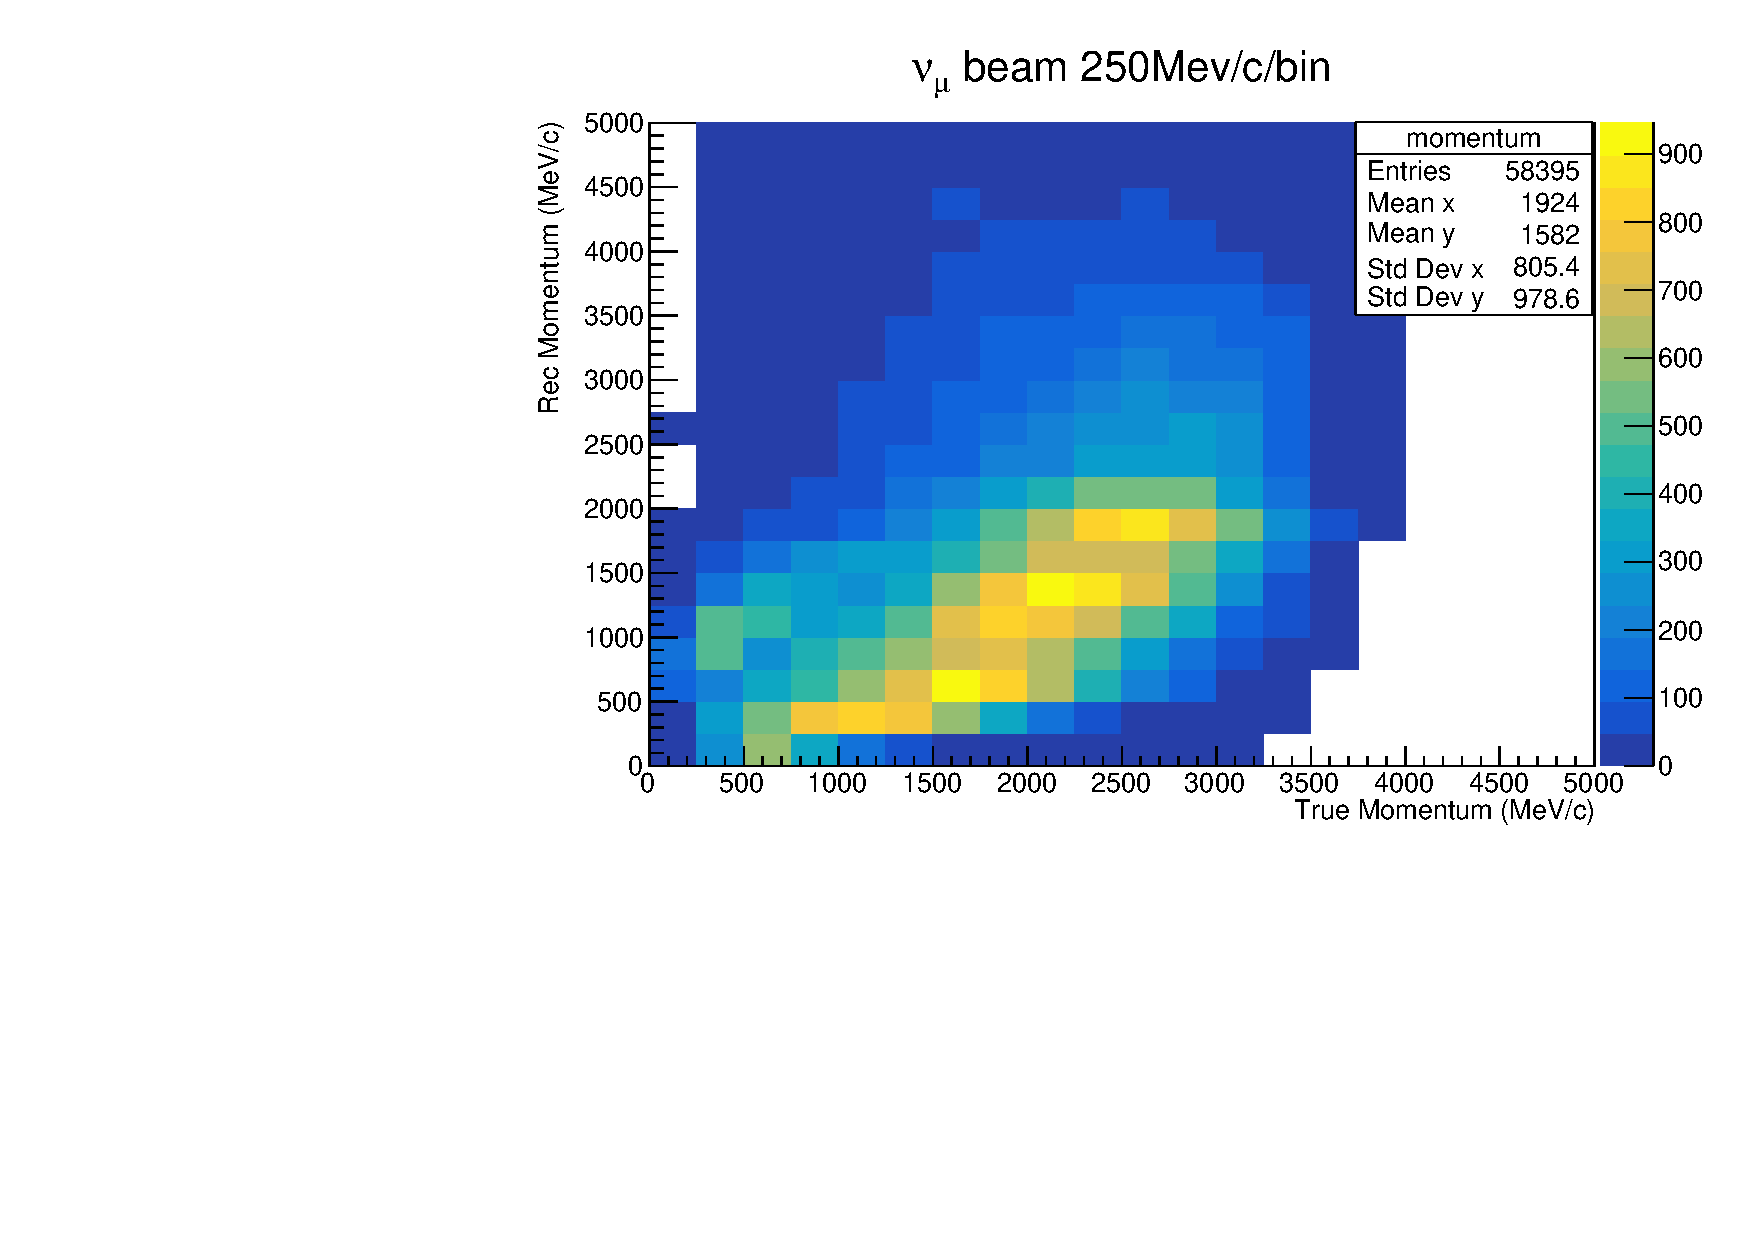
\includegraphics[width=\textwidth]{NuStorm/MomentumTASDNeutrinoBeamMIND.pdf}
		\end{figure}
	\end{column}%
	\begin{column}{.48\textwidth}
		\begin{figure}[h!]
			\centering
			%trim=l b r t
			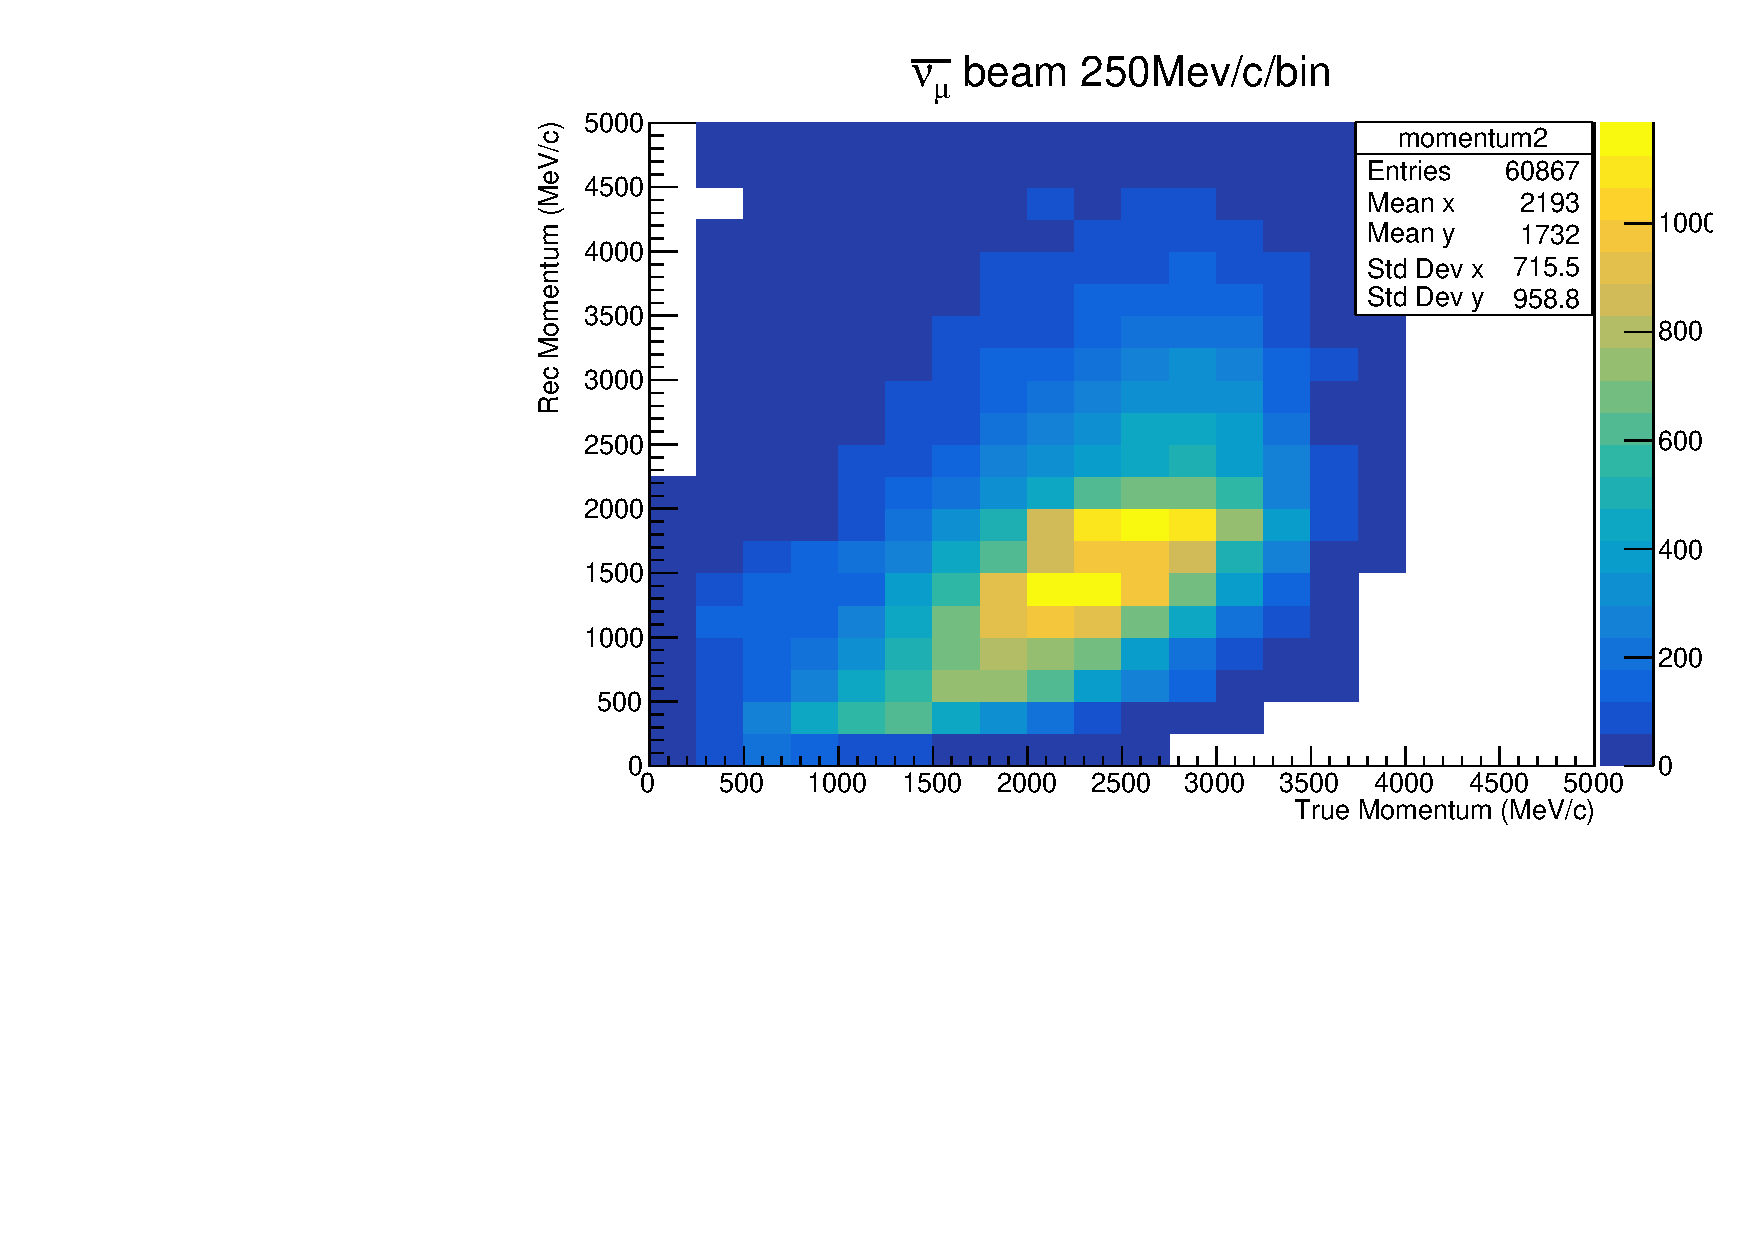
\includegraphics[width=\textwidth]{NuStorm/MomentumTASDAntiNeutrinoBeamMIND.pdf}
		\end{figure}
	\end{column}%
\end{columns}
\end{frame}

\begin{frame}{From the nuSTORM beam}
\begin{block}{}
	\begin{tiny}
		\begin{itemize}
			\item Interactions in TASD with NuStorm beam.
		\end{itemize}
	\end{tiny}
\end{block}
\begin{columns}[T] % align columns
	\begin{column}{.48\textwidth}
		
		\begin{figure}[h!]
			\centering
			%trim=l b r t
			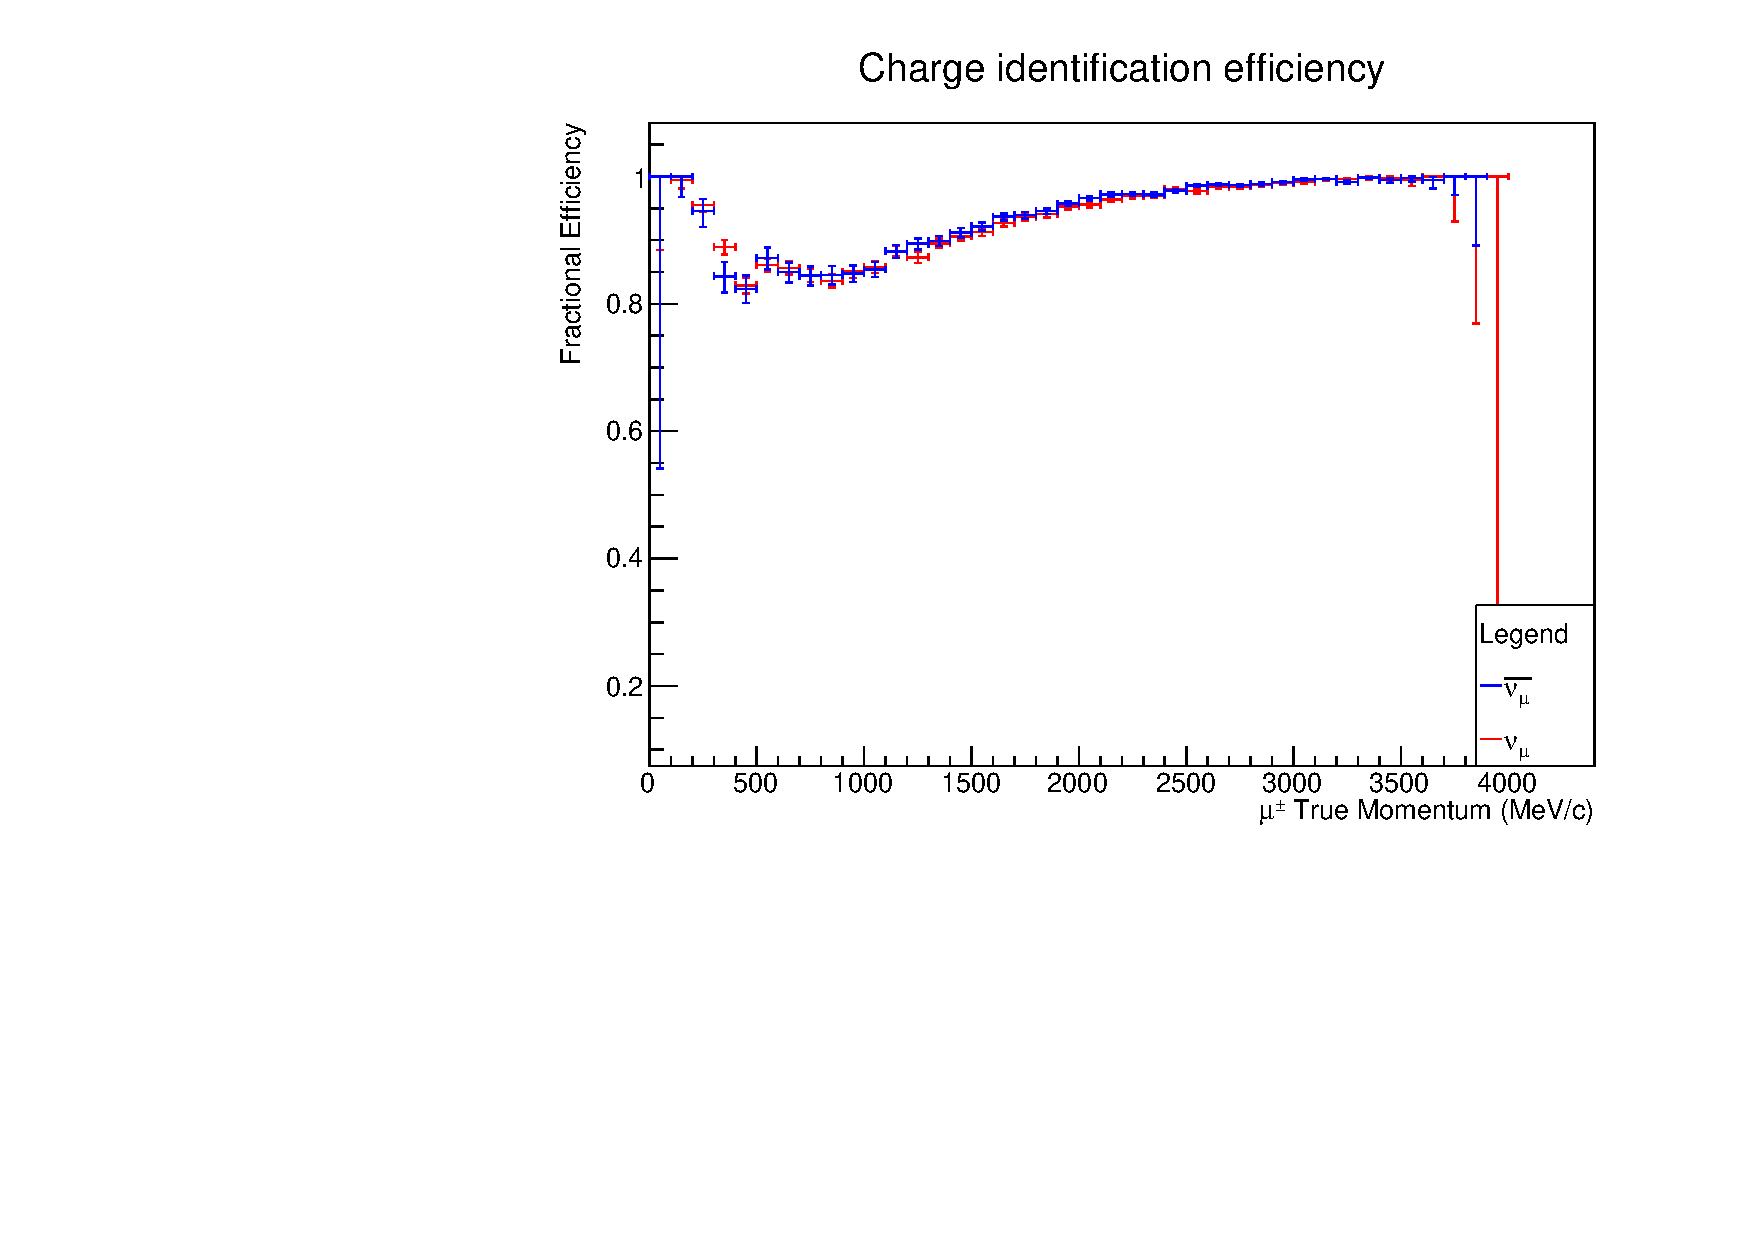
\includegraphics[width=\textwidth]{NuStorm/ChargeIDTASDNeutrinoBeamMIND.pdf}
		\end{figure}
	\end{column}%
	\begin{column}{.48\textwidth}
		\begin{figure}[h!]
			\centering
			%trim=l b r t
			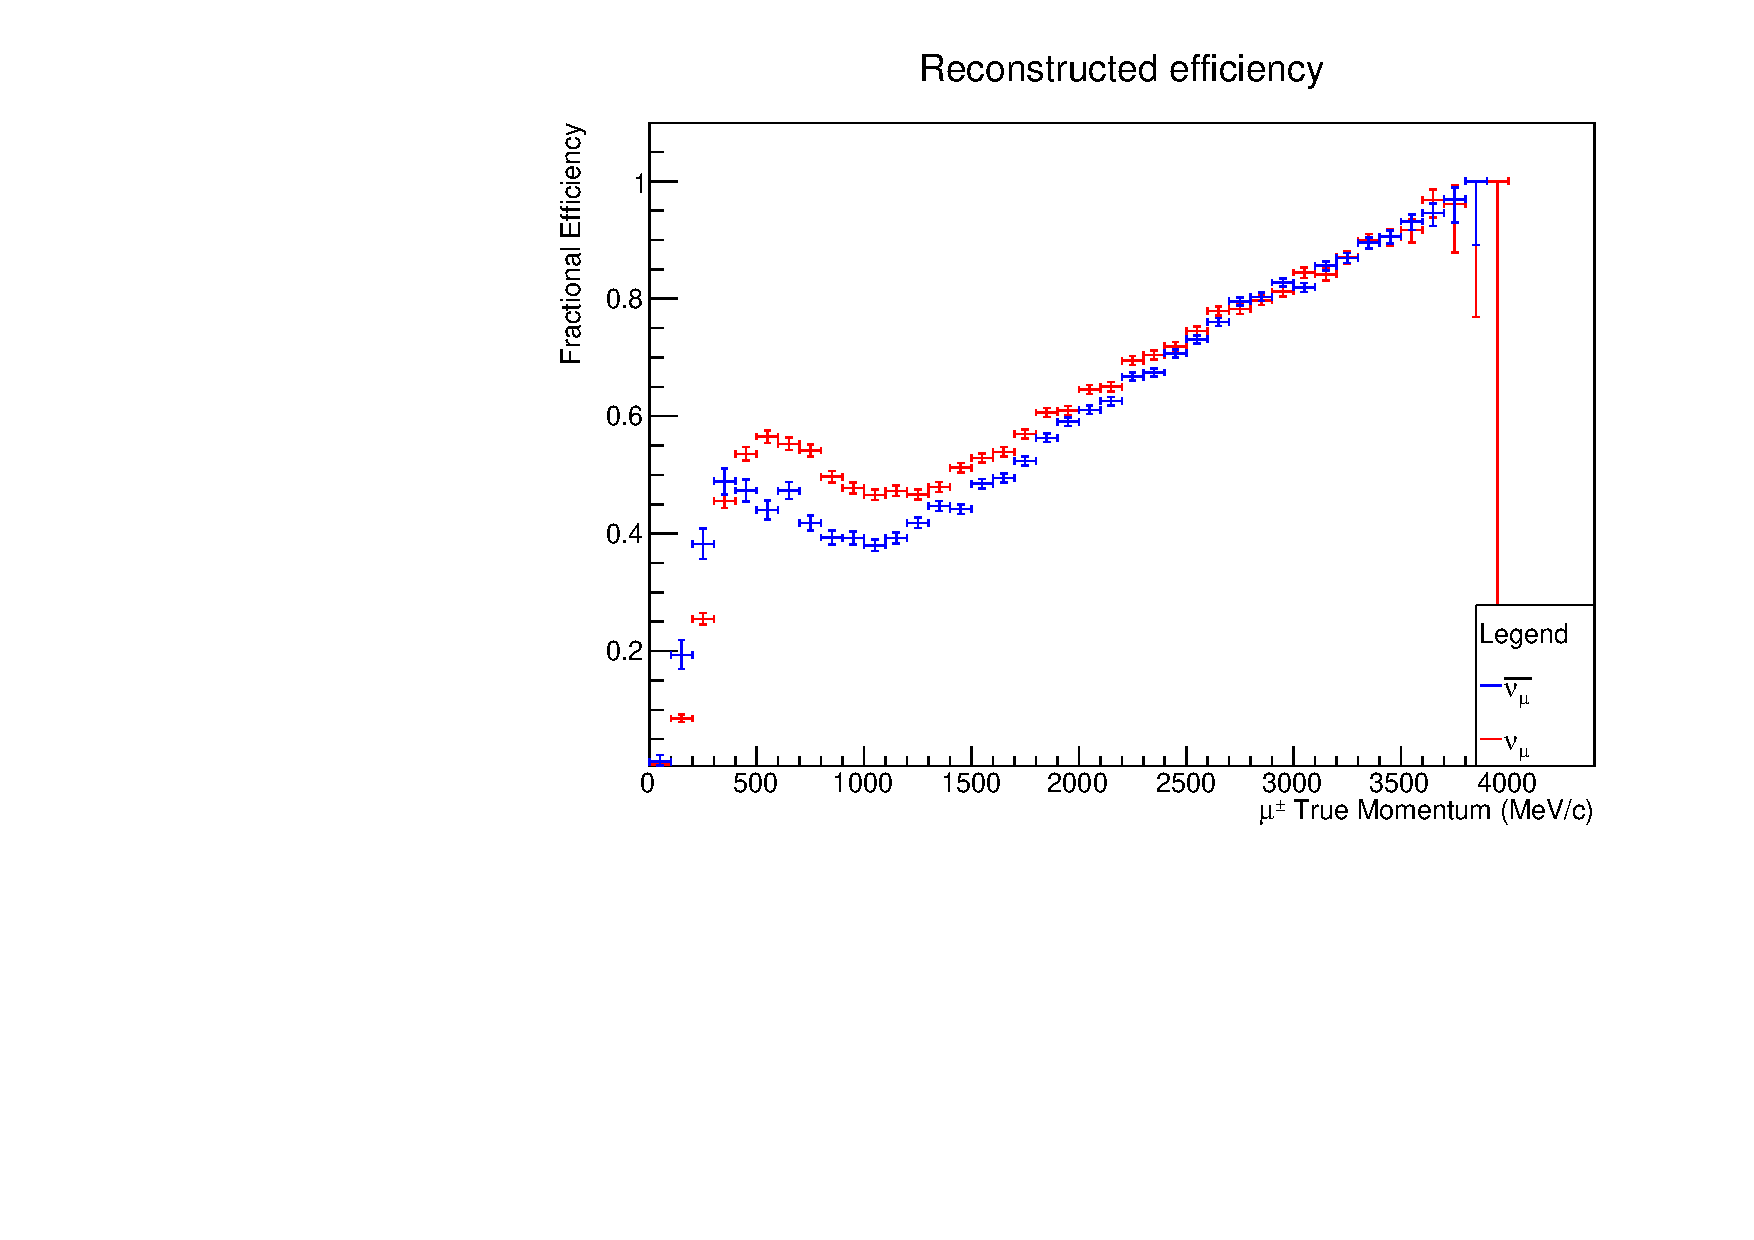
\includegraphics[width=\textwidth]{NuStorm/FittedTASDNeutrinoBeamMIND.pdf}
		\end{figure}
	\end{column}%
\end{columns}
\end{frame}

\begin{frame}{From the WAGASCI beam at 1.5 degrees}
\begin{block}{}
	\begin{tiny}
		\begin{itemize}
\item Show the neutrino and antineutrino spectra for the wrong-sign beam (also for the right-sign beam). Do the ratio of neutrino to antineutrino in bins of neutrino energy.
\item Do a GENIE simulation of the neutrino and antineutrino beam and place the events uniformly in the first three iron modules of Baby MIND. This will allow you to obtain the ratio of neutrino to antineutrino events (i.e.. multiplied by cross section) in Baby MIND as a function of neutrino energy.
\item This can be compared to the neutrino data from the last six days of data taking in May 2018. You can select neutrino events in Baby MIND by putting a veto on S1 and making a coincidence of S2 and S3 (or S4). This can be compared with the simulation. To avoid doing cross-sections, we do the ratio of neutrino to antineutrino (to first order, the nuclear effects in the cross sections cancel).

		\end{itemize}
	\end{tiny}
\end{block}

		\begin{figure}[h!]
	\centering
	%trim=l b r t
	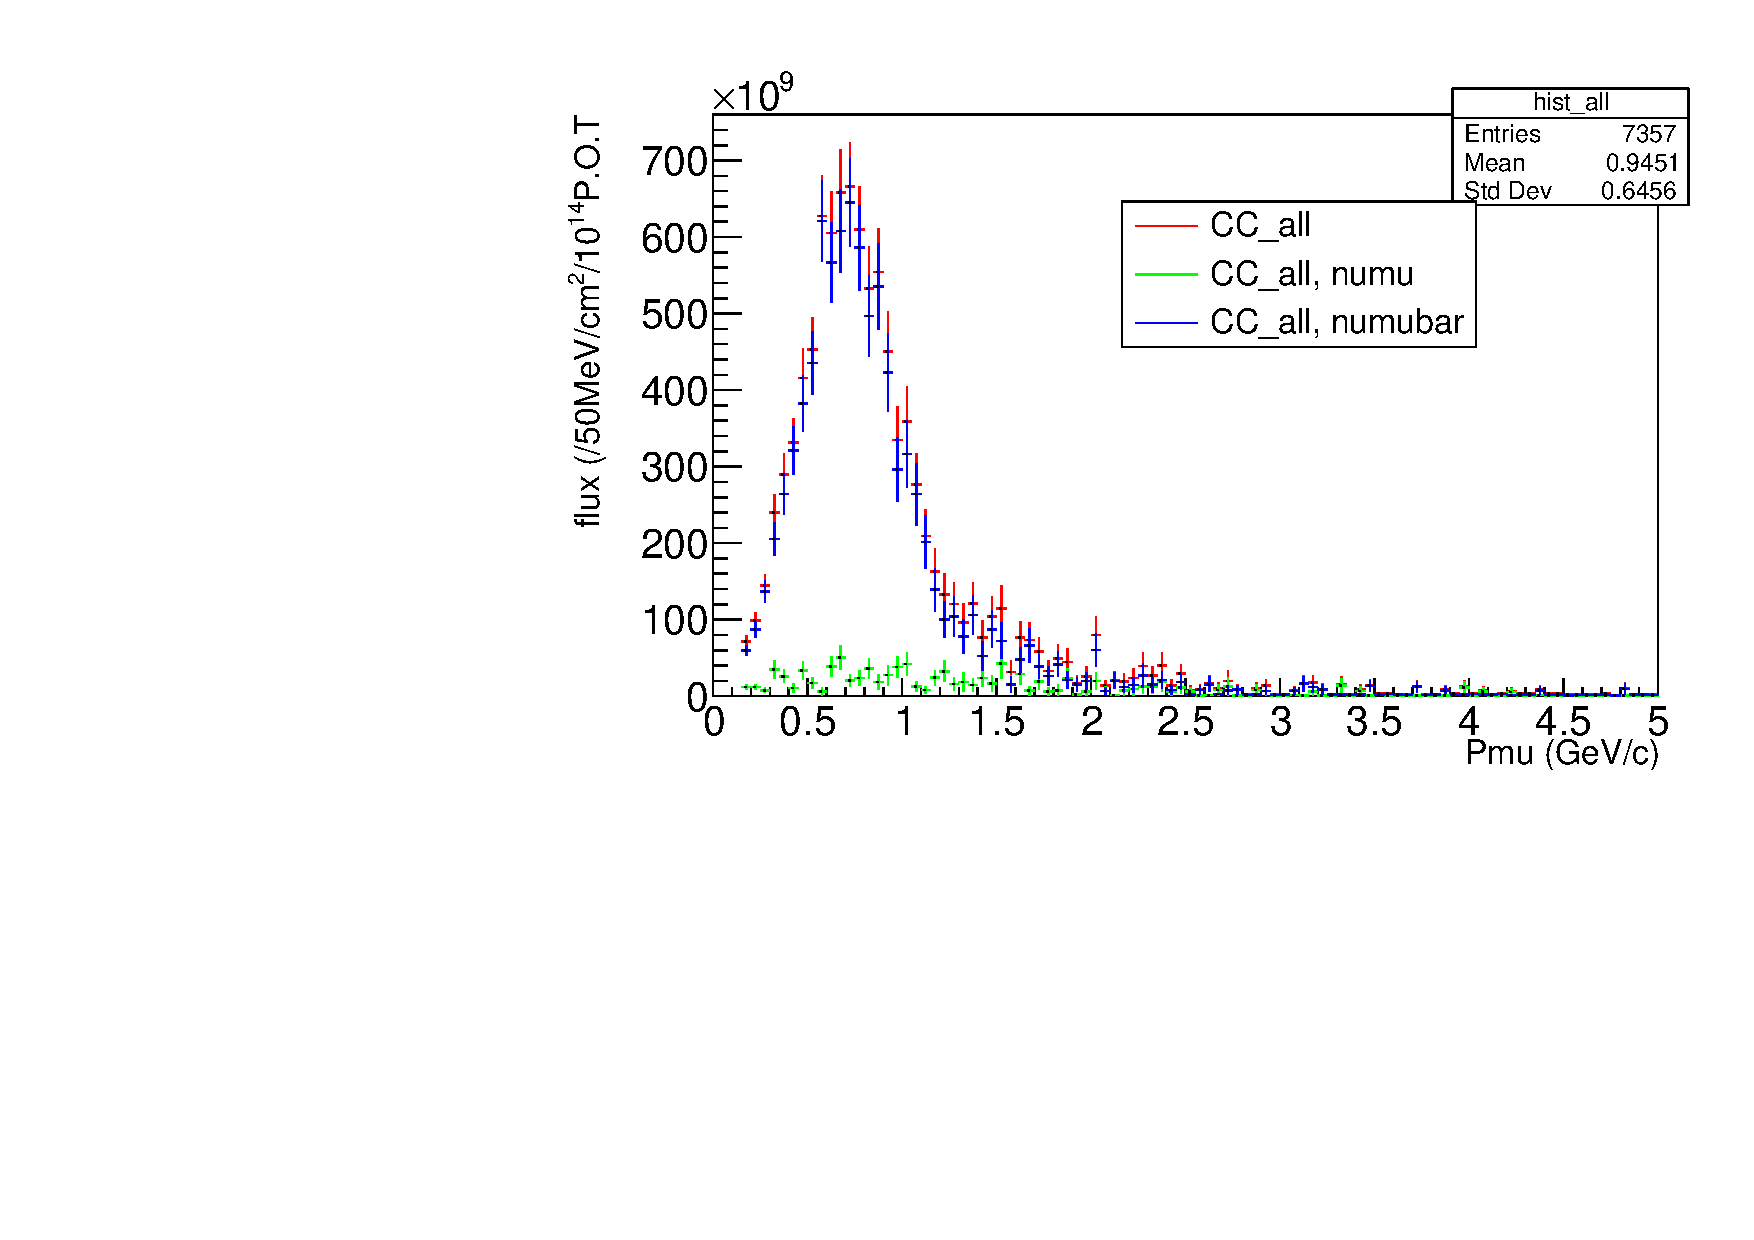
\includegraphics[width=.6\textwidth]{ND280Flux.pdf}
\end{figure}

\end{frame}

\begin{frame}{From the WAGASCI beam at 1.5 degrees}
\begin{columns}[T] % align columns
	\begin{column}{.48\textwidth}
		
		\begin{figure}[h!]
			\centering
			%trim=l b r t
			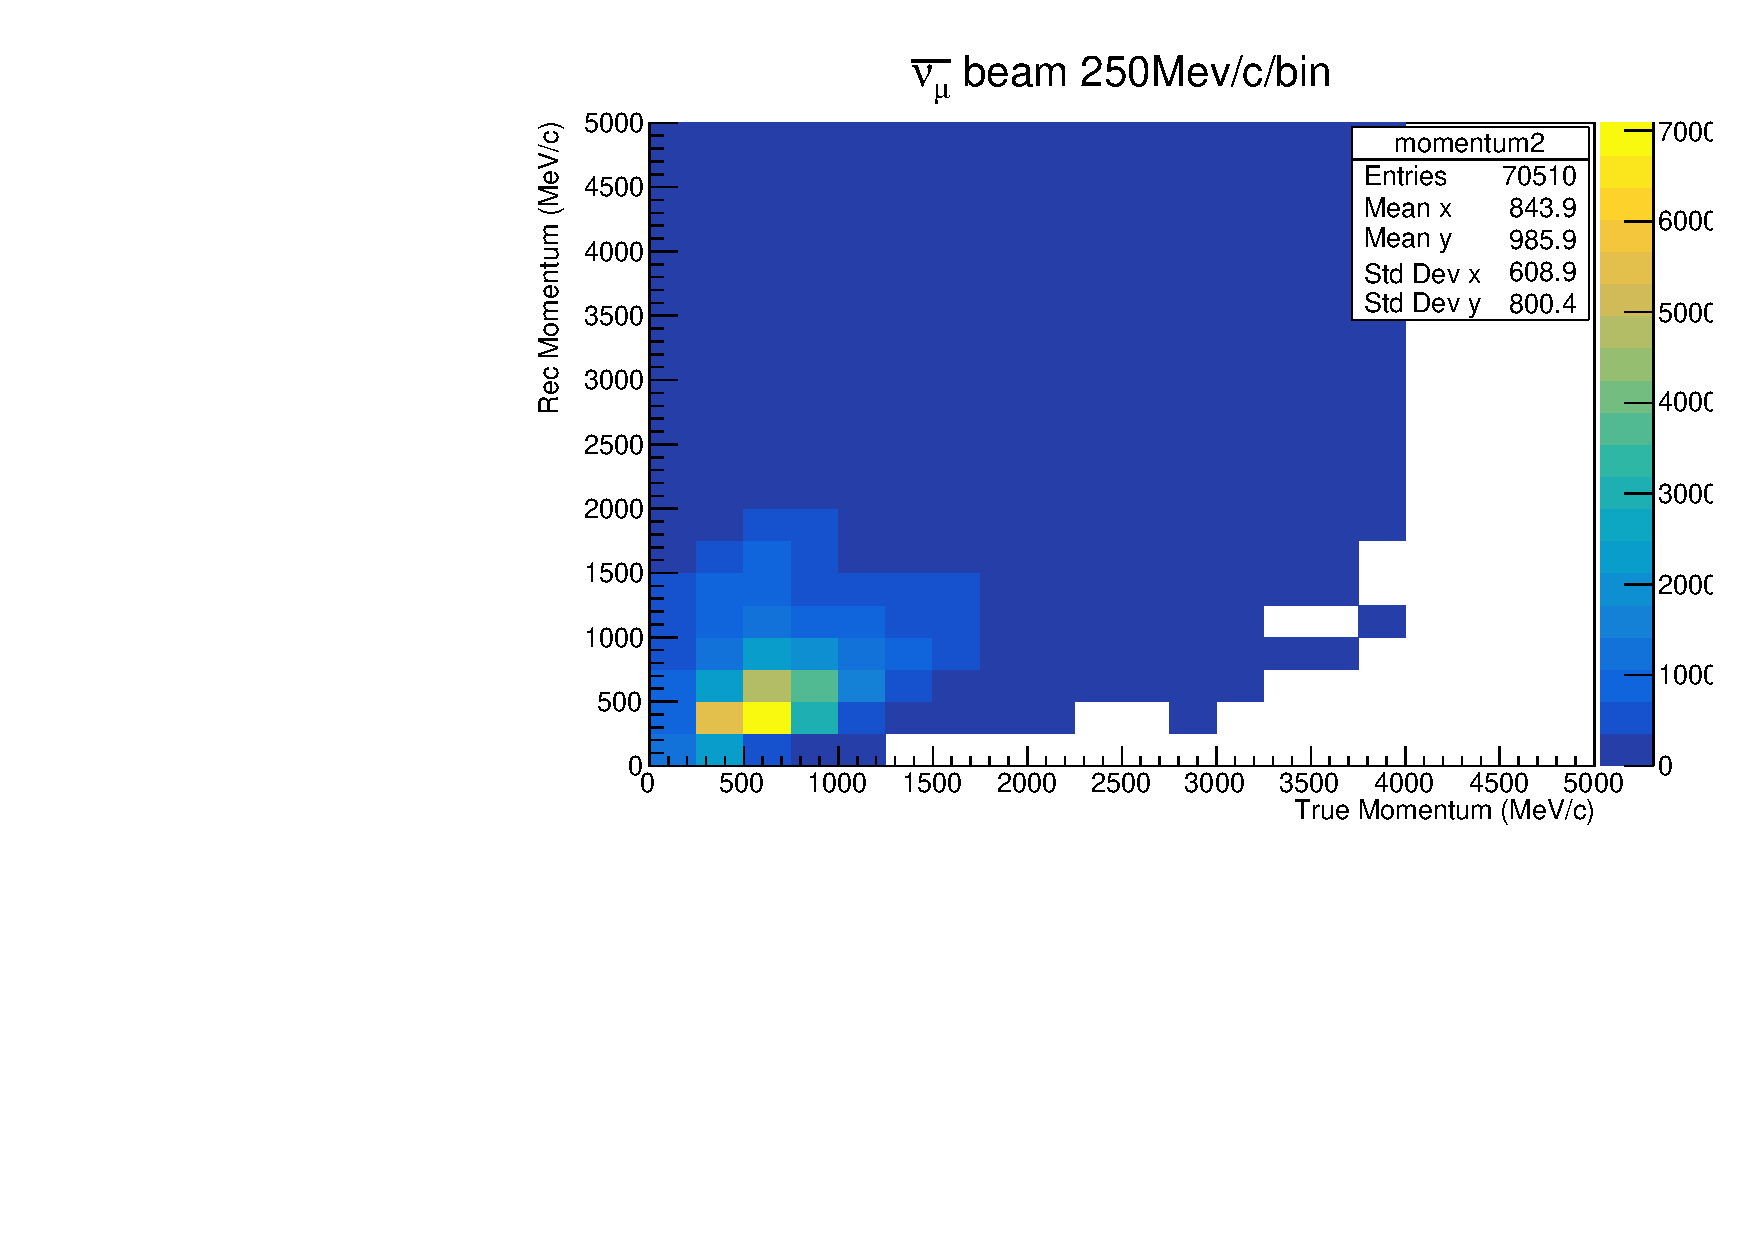
\includegraphics[width=.9\textwidth]{T2K/MomentumT2KAntiNeutrinoBeamMIND.pdf}
			
			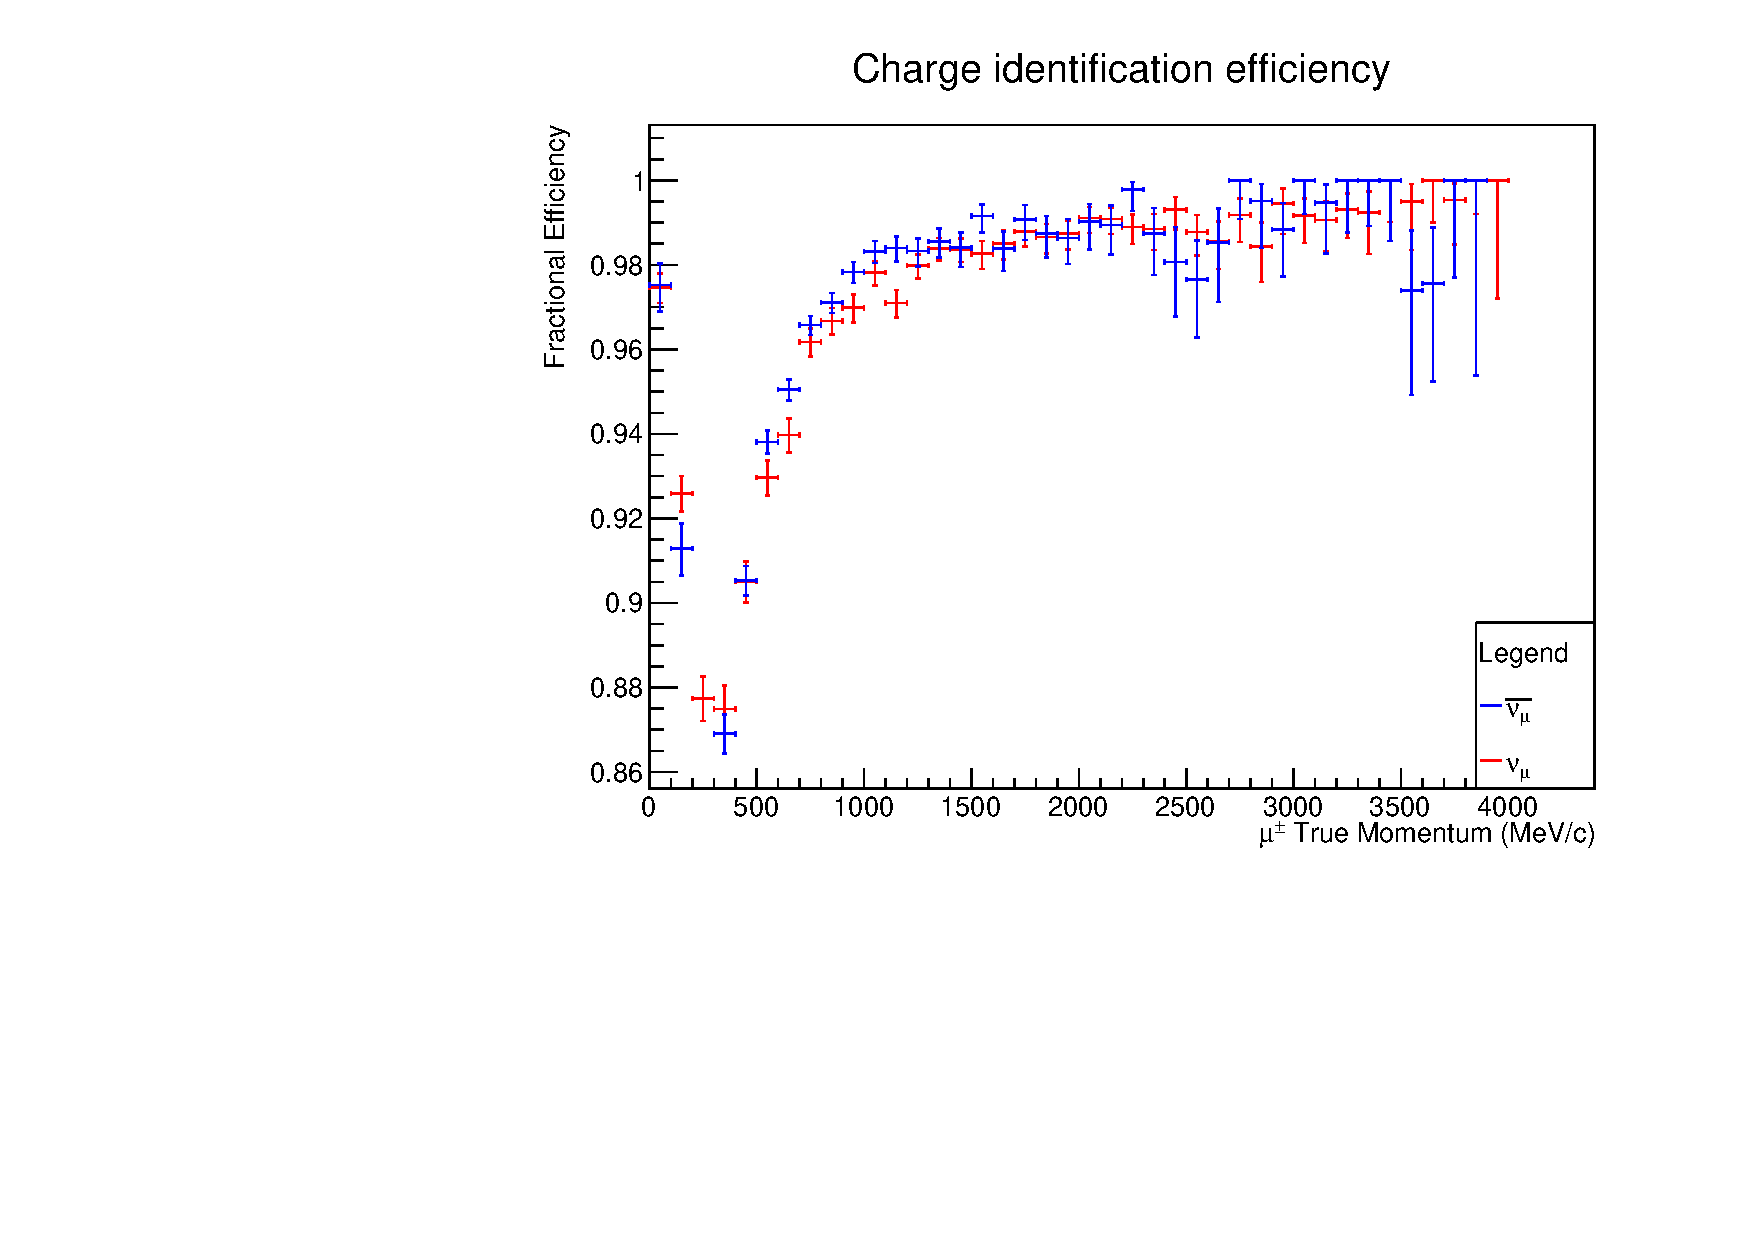
\includegraphics[width=.9\textwidth]{T2K/ChargeIDT2KNeutrinoBeamMIND.pdf}
		\end{figure}
	\end{column}%
	\begin{column}{.48\textwidth}
		\begin{figure}[h!]
			\centering
			%trim=l b r t
			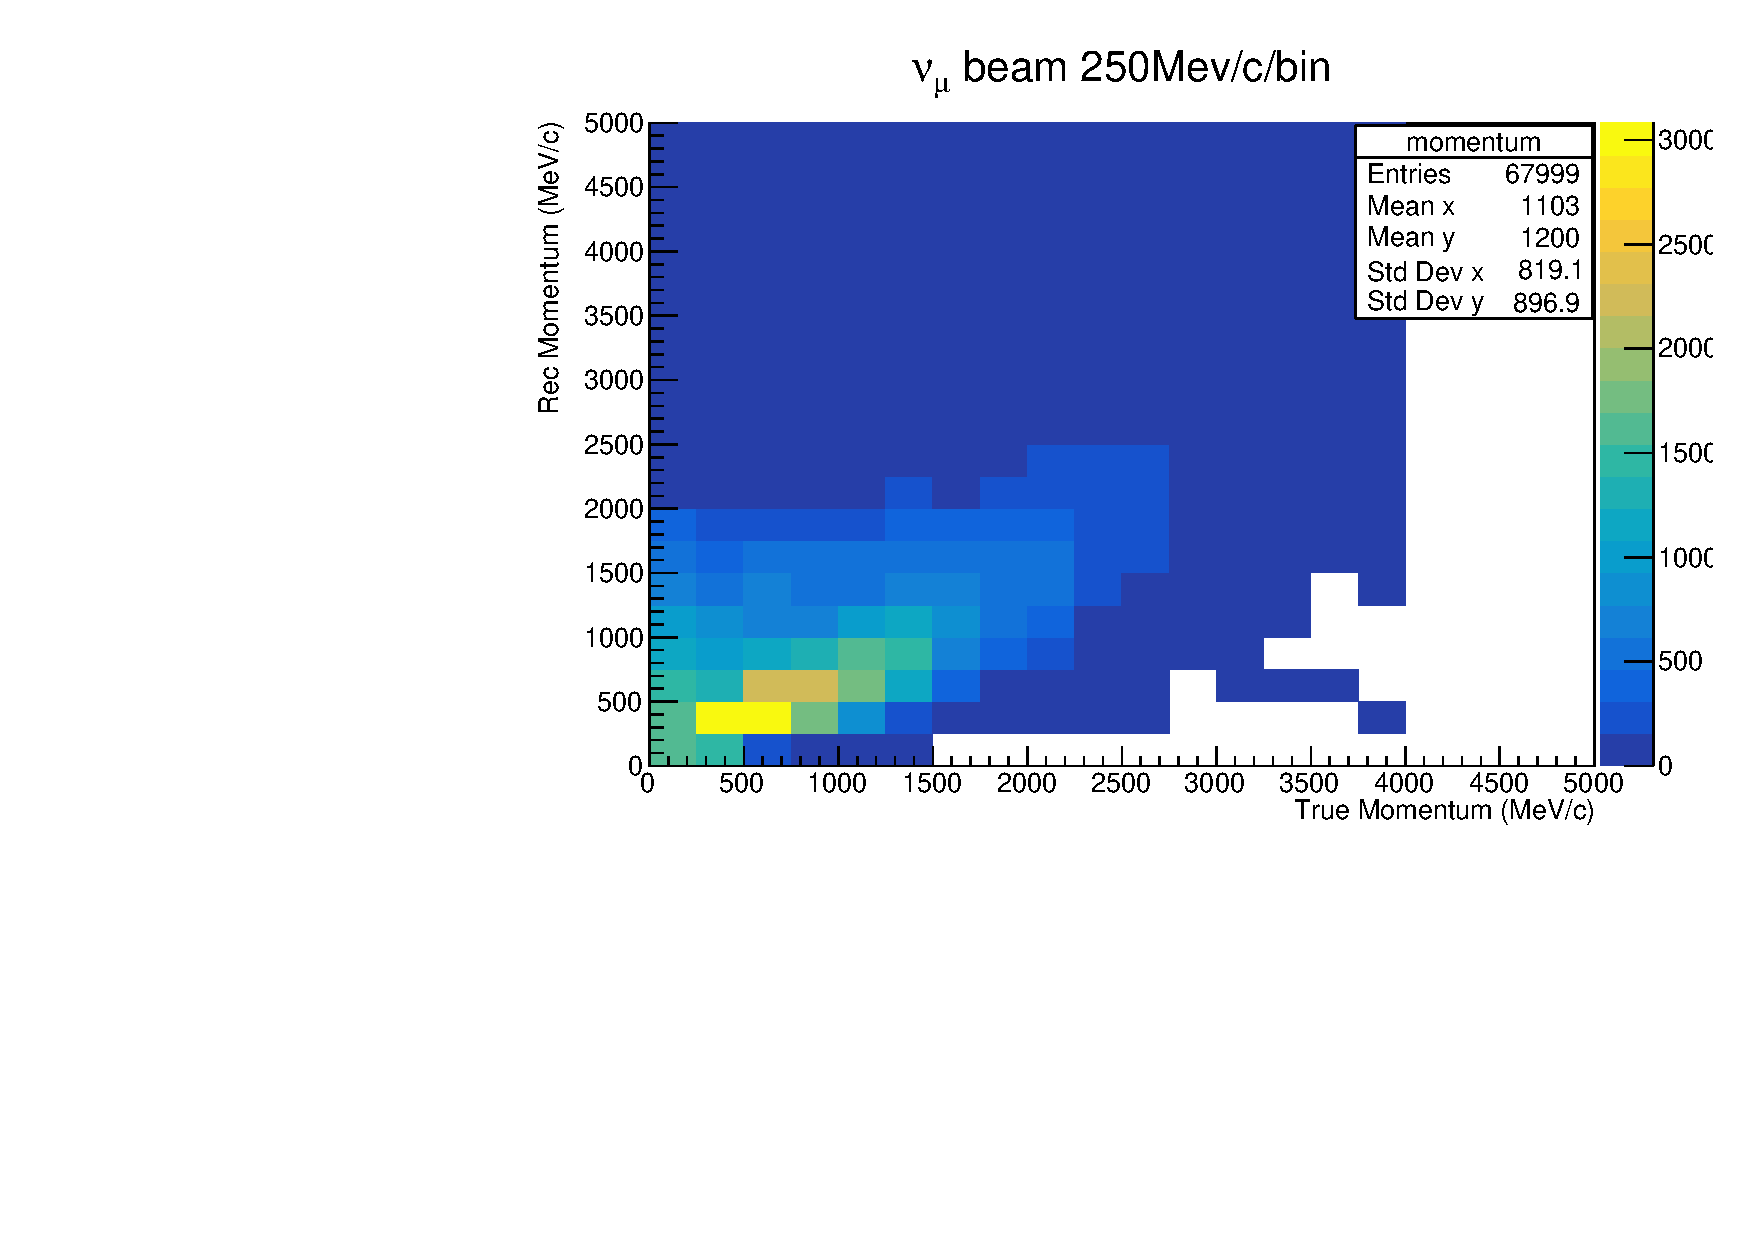
\includegraphics[width=.9\textwidth]{T2K/MomentumT2KNeutrinoBeamMIND.pdf}
			
			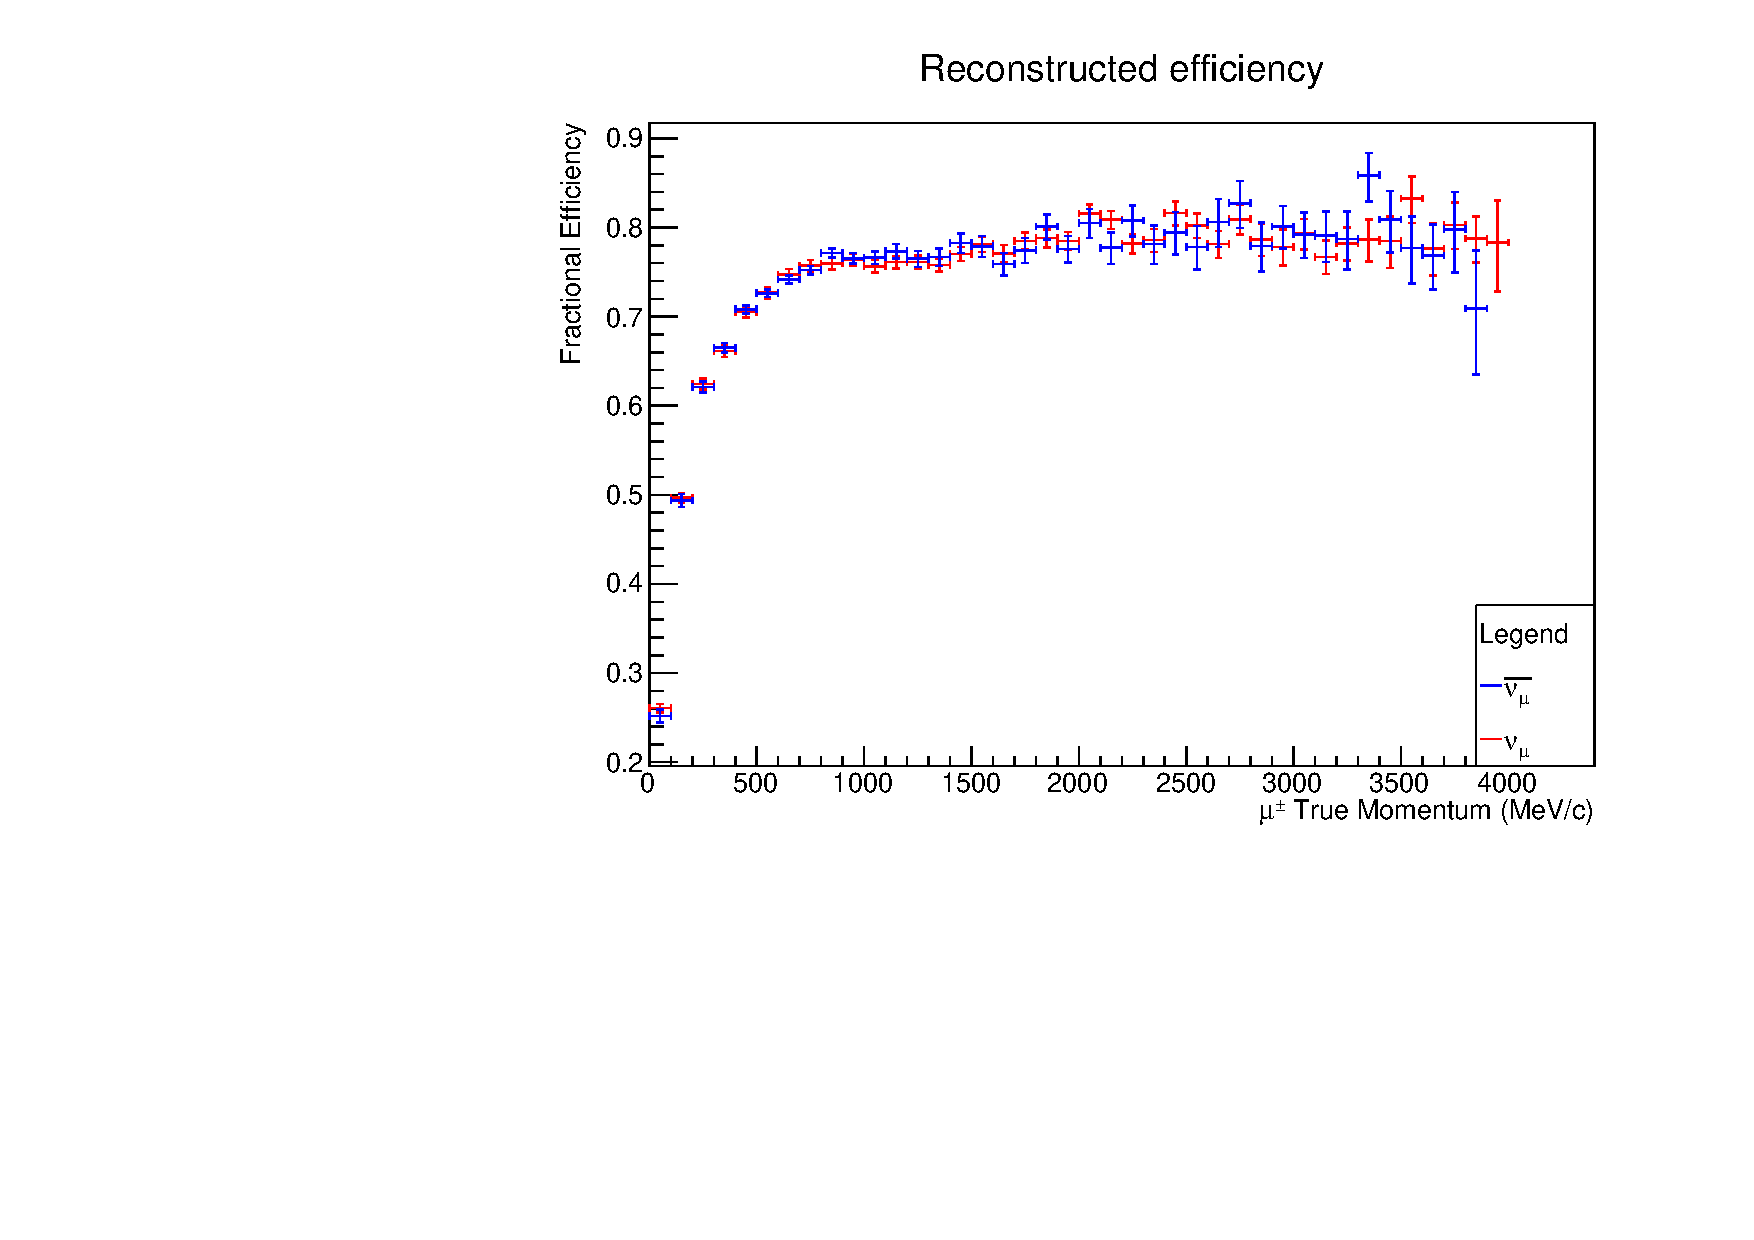
\includegraphics[width=.9\textwidth]{T2K/FittedT2KNeutrinoBeamMIND.pdf}
		\end{figure}
	\end{column}%
\end{columns}
\end{frame}

\end{document}